\documentclass{scrreprt}\usepackage[]{graphicx}\usepackage[]{color}
%% maxwidth is the original width if it is less than linewidth
%% otherwise use linewidth (to make sure the graphics do not exceed the margin)
\makeatletter
\def\maxwidth{ %
  \ifdim\Gin@nat@width>\linewidth
    \linewidth
  \else
    \Gin@nat@width
  \fi
}
\makeatother

\definecolor{fgcolor}{rgb}{0.345, 0.345, 0.345}
\newcommand{\hlnum}[1]{\textcolor[rgb]{0.686,0.059,0.569}{#1}}%
\newcommand{\hlstr}[1]{\textcolor[rgb]{0.192,0.494,0.8}{#1}}%
\newcommand{\hlcom}[1]{\textcolor[rgb]{0.678,0.584,0.686}{\textit{#1}}}%
\newcommand{\hlopt}[1]{\textcolor[rgb]{0,0,0}{#1}}%
\newcommand{\hlstd}[1]{\textcolor[rgb]{0.345,0.345,0.345}{#1}}%
\newcommand{\hlkwa}[1]{\textcolor[rgb]{0.161,0.373,0.58}{\textbf{#1}}}%
\newcommand{\hlkwb}[1]{\textcolor[rgb]{0.69,0.353,0.396}{#1}}%
\newcommand{\hlkwc}[1]{\textcolor[rgb]{0.333,0.667,0.333}{#1}}%
\newcommand{\hlkwd}[1]{\textcolor[rgb]{0.737,0.353,0.396}{\textbf{#1}}}%

\usepackage{framed}
\makeatletter
\newenvironment{kframe}{%
 \def\at@end@of@kframe{}%
 \ifinner\ifhmode%
  \def\at@end@of@kframe{\end{minipage}}%
  \begin{minipage}{\columnwidth}%
 \fi\fi%
 \def\FrameCommand##1{\hskip\@totalleftmargin \hskip-\fboxsep
 \colorbox{shadecolor}{##1}\hskip-\fboxsep
     % There is no \\@totalrightmargin, so:
     \hskip-\linewidth \hskip-\@totalleftmargin \hskip\columnwidth}%
 \MakeFramed {\advance\hsize-\width
   \@totalleftmargin\z@ \linewidth\hsize
   \@setminipage}}%
 {\par\unskip\endMakeFramed%
 \at@end@of@kframe}
\makeatother

\definecolor{shadecolor}{rgb}{.97, .97, .97}
\definecolor{messagecolor}{rgb}{0, 0, 0}
\definecolor{warningcolor}{rgb}{1, 0, 1}
\definecolor{errorcolor}{rgb}{1, 0, 0}
\newenvironment{knitrout}{}{} % an empty environment to be redefined in TeX

\usepackage{alltt}
\usepackage[a3paper,twocolumn]{geometry}
\IfFileExists{upquote.sty}{\usepackage{upquote}}{}
\begin{document}
\begin{knitrout}
\definecolor{shadecolor}{rgb}{0.969, 0.969, 0.969}\color{fgcolor}\begin{kframe}
\begin{alltt}
\hlkwd{library}\hlstd{(knitr)}
\hlstd{.finished} \hlkwb{<-} \hlnum{FALSE}
\hlstd{knit_hooks}\hlopt{$}\hlkwd{set}\hlstd{(}\hlkwc{timeit} \hlstd{=} \hlkwa{function}\hlstd{(}\hlkwc{before}\hlstd{) \{}
    \hlkwa{if} \hlstd{(before) \{}
      \hlstd{.current.time} \hlkwb{<<-} \hlkwd{Sys.time}\hlstd{()}
    \hlstd{\}} \hlkwa{else} \hlstd{\{}
      \hlstd{.duration} \hlkwb{<-} \hlkwd{round}\hlstd{(}\hlkwd{difftime}\hlstd{(}\hlkwd{Sys.time}\hlstd{(), .current.time,} \hlkwc{units} \hlstd{=} \hlstr{"secs"}\hlstd{))}
      \hlkwa{if}\hlstd{(}\hlopt{!}\hlstd{.finished)}
        \hlkwd{write}\hlstd{(}
          \hlkwd{paste0}\hlstd{(}
            \hlstd{knitr}\hlopt{::}\hlstd{opts_current}\hlopt{$}\hlkwd{get}\hlstd{(}\hlkwc{name} \hlstd{=} \hlstr{"label"}\hlstd{),}
            \hlstr{": "}\hlstd{,}
            \hlstd{.duration),}
          \hlkwc{file} \hlstd{=} \hlstr{"analysis-post-2008-CHUNKTIMINGS.txt"}\hlstd{,}
          \hlkwc{ncolumns} \hlstd{=} \hlnum{1}\hlstd{,}
          \hlkwc{append} \hlstd{=} \hlnum{TRUE}\hlstd{)}
    \hlstd{\}}
\hlstd{\})}
\hlkwd{file.remove}\hlstd{(}\hlstr{"analysis-post-2008-CHUNKTIMINGS.txt"}\hlstd{)}
\end{alltt}
\begin{verbatim}
## [1] TRUE
\end{verbatim}
\begin{alltt}
\hlstd{START.TIME} \hlkwb{<-} \hlkwd{Sys.time}\hlstd{()}
\hlstd{knitr}\hlopt{::}\hlstd{opts_chunk}\hlopt{$}\hlkwd{set}\hlstd{(}\hlkwc{fig.show} \hlstd{=} \hlstr{'hide'}\hlstd{,}
                      \hlkwc{fig.width} \hlstd{=} \hlnum{11}\hlstd{,}
                      \hlkwc{fig.height} \hlstd{=} \hlnum{7}\hlstd{,}
                      \hlkwc{fig.path} \hlstd{= atlas} \hlkwb{<-} \hlstr{"atlas-post-2008/"}\hlstd{,}
                      \hlkwc{timeit} \hlstd{=} \hlnum{TRUE}\hlstd{,}
                      \hlkwc{cache}\hlstd{=}\hlnum{FALSE}\hlstd{,}
                      \hlkwc{out.width} \hlstd{=} \hlstr{"11in"}\hlstd{)}
\end{alltt}
\end{kframe}
\end{knitrout}

\begin{knitrout}
\definecolor{shadecolor}{rgb}{0.969, 0.969, 0.969}\color{fgcolor}\begin{kframe}
\begin{alltt}
\hlkwd{library}\hlstd{(tidyr)}
\hlkwd{library}\hlstd{(data.table)}
\hlkwd{library}\hlstd{(bit64)}
\end{alltt}


{\ttfamily\noindent\itshape\color{messagecolor}{\#\# Loading required package: bit\\\#\# Attaching package bit\\\#\# package:bit (c) 2008-2012 Jens Oehlschlaegel (GPL-2)\\\#\# creators: bit bitwhich\\\#\# coercion: as.logical as.integer as.bit as.bitwhich which\\\#\# operator: ! \& | xor != ==\\\#\# querying: print length any all min max range sum summary\\\#\# bit access: length<- [ [<- [[ [[<-\\\#\# for more help type ?bit\\\#\# \\\#\# Attaching package: 'bit'\\\#\# \\\#\# The following object is masked from 'package:data.table':\\\#\# \\\#\#\ \ \ \  setattr\\\#\# \\\#\# The following object is masked from 'package:base':\\\#\# \\\#\#\ \ \ \  xor\\\#\# \\\#\# Attaching package bit64\\\#\# package:bit64 (c) 2011-2012 Jens Oehlschlaegel (GPL-2 with commercial restrictions)\\\#\# creators: integer64 seq :\\\#\# coercion: as.integer64 as.vector as.logical as.integer as.double as.character as.bin\\\#\# logical operator: ! \& | xor != == < <= >= >\\\#\# arithmetic operator: + - * / \%/\% \%\% \textasciicircum{}\\\#\# math: sign abs sqrt log log2 log10\\\#\# math: floor ceiling trunc round\\\#\# querying: is.integer64 is.vector [is.atomic\} [length] is.na format print\\\#\# aggregation: any all min max range sum prod\\\#\# cumulation: diff cummin cummax cumsum cumprod\\\#\# access: length<- [ [<- [[ [[<-\\\#\# combine: c rep cbind rbind as.data.frame\\\#\# for more help type ?bit64\\\#\# \\\#\# Attaching package: 'bit64'\\\#\# \\\#\# The following object is masked from 'package:bit':\\\#\# \\\#\#\ \ \ \  still.identical\\\#\# \\\#\# The following objects are masked from 'package:base':\\\#\# \\\#\#\ \ \ \  \%in\%, :, is.double, match, order, rank}}\begin{alltt}
\hlkwd{library}\hlstd{(dplyr)}
\end{alltt}


{\ttfamily\noindent\itshape\color{messagecolor}{\#\# \\\#\# Attaching package: 'dplyr'\\\#\# \\\#\# The following objects are masked from 'package:data.table':\\\#\# \\\#\#\ \ \ \  between, last\\\#\# \\\#\# The following objects are masked from 'package:stats':\\\#\# \\\#\#\ \ \ \  filter, lag\\\#\# \\\#\# The following objects are masked from 'package:base':\\\#\# \\\#\#\ \ \ \  intersect, setdiff, setequal, union}}\begin{alltt}
\hlkwd{library}\hlstd{(magrittr)}
\end{alltt}


{\ttfamily\noindent\itshape\color{messagecolor}{\#\# \\\#\# Attaching package: 'magrittr'\\\#\# \\\#\# The following object is masked from 'package:tidyr':\\\#\# \\\#\#\ \ \ \  extract}}\begin{alltt}
\hlkwd{library}\hlstd{(ggplot2)}
\hlstd{theme.text.size} \hlkwb{=} \hlnum{18}
\hlstd{text.size} \hlkwb{=} \hlstd{(}\hlnum{5}\hlopt{/}\hlnum{14}\hlstd{)} \hlopt{*} \hlstd{theme.text.size}
\hlkwd{theme_update}\hlstd{(}\hlkwc{text} \hlstd{=} \hlkwd{element_text}\hlstd{(}\hlkwc{family} \hlstd{=} \hlstr{""}\hlstd{,}
                                 \hlkwc{face} \hlstd{=} \hlstr{"plain"}\hlstd{,} \hlkwc{colour} \hlstd{=} \hlstr{"black"}\hlstd{,} \hlkwc{size} \hlstd{= theme.text.size,}
                                 \hlkwc{lineheight} \hlstd{=} \hlnum{0.9}\hlstd{,}
                                 \hlkwc{hjust} \hlstd{=} \hlnum{0.5}\hlstd{,} \hlkwc{vjust} \hlstd{=} \hlnum{0.5}\hlstd{,}
                                 \hlkwc{angle} \hlstd{=} \hlnum{0}\hlstd{,} \hlkwc{margin} \hlstd{=} \hlkwd{margin}\hlstd{(),}
                                 \hlkwc{debug} \hlstd{=} \hlnum{FALSE}\hlstd{))}
\hlkwd{update_geom_defaults}\hlstd{(}\hlstr{"text"}\hlstd{,} \hlkwd{list}\hlstd{(}\hlkwc{size} \hlstd{= text.size))}
\hlkwd{update_geom_defaults}\hlstd{(}\hlstr{"line"}\hlstd{,} \hlkwd{list}\hlstd{(}\hlkwc{size} \hlstd{=} \hlnum{2}\hlstd{))}
\hlkwd{library}\hlstd{(ggrepel)}
\hlkwd{library}\hlstd{(scales)}
\hlkwd{library}\hlstd{(nycflights13)}  \hlcom{# for airports}
\hlstd{nycflights.airports} \hlkwb{<-} \hlstd{airports}
\hlstd{nycflights.planes}   \hlkwb{<-} \hlstd{planes}
\hlstd{nycflights.airlines} \hlkwb{<-} \hlkwd{as.data.table}\hlstd{(airlines)}
\hlkwa{for} \hlstd{(j} \hlkwa{in} \hlnum{1}\hlopt{:}\hlkwd{ncol}\hlstd{(nycflights.airlines))\{}
  \hlkwd{set}\hlstd{(nycflights.airlines,} \hlkwc{j} \hlstd{= j,} \hlkwc{value} \hlstd{=} \hlkwd{as.character}\hlstd{(nycflights.airlines[[j]]))}
\hlstd{\}}
\hlstd{nycflights.airlines[,short_name} \hlkwb{:=} \hlkwd{gsub}\hlstd{(}\hlstr{"\textbackslash{}\textbackslash{}s.*$"}\hlstd{,} \hlstr{""}\hlstd{, name)]}
\hlkwd{setnames}\hlstd{(nycflights.airlines,} \hlstr{"carrier"}\hlstd{,} \hlstr{"UniqueCarrier"}\hlstd{)}
\hlkwd{setkey}\hlstd{(nycflights.airlines, UniqueCarrier)}
\hlkwd{library}\hlstd{(fasttime)}
\hlkwd{library}\hlstd{(grattan)}
\end{alltt}


{\ttfamily\noindent\itshape\color{messagecolor}{\#\# \\\#\# Attaching package: 'grattan'\\\#\# \\\#\# The following object is masked from 'package:datasets':\\\#\# \\\#\#\ \ \ \  Orange}}\begin{alltt}
\hlkwd{library}\hlstd{(directlabels)}
\hlkwd{library}\hlstd{(ineq)}  \hlcom{# for Gini()}
\end{alltt}
\end{kframe}
\end{knitrout}

\begin{knitrout}
\definecolor{shadecolor}{rgb}{0.969, 0.969, 0.969}\color{fgcolor}\begin{kframe}
\begin{alltt}
\hlstd{convert_week_to_date} \hlkwb{<-} \hlkwa{function}\hlstd{(}\hlkwc{DT_with_Week_column}\hlstd{,} \hlkwc{override} \hlstd{=} \hlnum{FALSE}\hlstd{)\{}
  \hlkwd{stopifnot}\hlstd{(}\hlkwd{is.data.table}\hlstd{(DT_with_Week_column),} \hlstr{"Week"} \hlopt \hlkwd{names}\hlstd{(DT_with_Week_column))}
  \hlkwd{setkey}\hlstd{(DT_with_Week_column, Week)}
  \hlstd{temp} \hlkwb{<-}
    \hlstd{unique_dates} \hlopt
    \hlkwd{group_by}\hlstd{(Week)} \hlopt
    \hlkwd{summarise}\hlstd{(}\hlkwc{Date} \hlstd{=} \hlkwd{fastPOSIXct}\hlstd{(}\hlkwd{sprintf}\hlstd{(}\hlstr{"%d-%02d-%02d"}\hlstd{,} \hlkwd{first}\hlstd{(Year),} \hlkwd{first}\hlstd{(Month),} \hlkwd{first}\hlstd{(DayofMonth))))} \hlopt
    \hlkwd{setkey}\hlstd{(Week)}

  \hlstd{DT_with_Week_column[temp]}
\hlstd{\}}
\end{alltt}
\end{kframe}
\end{knitrout}

\begin{knitrout}
\definecolor{shadecolor}{rgb}{0.969, 0.969, 0.969}\color{fgcolor}\begin{kframe}
\begin{alltt}
\hlstd{flights} \hlkwb{<-} \hlkwd{fread}\hlstd{(}\hlstr{"../post2008_flights.csv"}\hlstd{,} \hlkwc{na.strings} \hlstd{=} \hlkwd{c}\hlstd{(}\hlstr{"NA"}\hlstd{,} \hlstr{""}\hlstd{))}
\end{alltt}
\begin{verbatim}
## 
Read 0.0% of 49153341 rows
Read 0.7% of 49153341 rows
Read 1.4% of 49153341 rows
Read 2.0% of 49153341 rows
Read 2.7% of 49153341 rows
Read 3.4% of 49153341 rows
Read 4.1% of 49153341 rows
Read 4.8% of 49153341 rows
Read 5.5% of 49153341 rows
Read 6.2% of 49153341 rows
Read 6.9% of 49153341 rows
Read 7.5% of 49153341 rows
Read 8.2% of 49153341 rows
Read 8.9% of 49153341 rows
Read 9.6% of 49153341 rows
Read 10.3% of 49153341 rows
Read 11.0% of 49153341 rows
Read 11.7% of 49153341 rows
Read 12.3% of 49153341 rows
Read 13.0% of 49153341 rows
Read 13.7% of 49153341 rows
Read 14.4% of 49153341 rows
Read 15.1% of 49153341 rows
Read 15.8% of 49153341 rows
Read 16.5% of 49153341 rows
Read 17.2% of 49153341 rows
Read 17.9% of 49153341 rows
Read 18.6% of 49153341 rows
Read 19.3% of 49153341 rows
Read 20.0% of 49153341 rows
Read 20.6% of 49153341 rows
Read 21.3% of 49153341 rows
Read 22.0% of 49153341 rows
Read 22.7% of 49153341 rows
Read 23.4% of 49153341 rows
Read 24.1% of 49153341 rows
Read 24.8% of 49153341 rows
Read 25.5% of 49153341 rows
Read 26.2% of 49153341 rows
Read 26.9% of 49153341 rows
Read 27.6% of 49153341 rows
Read 28.3% of 49153341 rows
Read 29.0% of 49153341 rows
Read 29.6% of 49153341 rows
Read 30.3% of 49153341 rows
Read 31.0% of 49153341 rows
Read 31.7% of 49153341 rows
Read 32.4% of 49153341 rows
Read 33.1% of 49153341 rows
Read 33.8% of 49153341 rows
Read 34.5% of 49153341 rows
Read 35.2% of 49153341 rows
Read 35.8% of 49153341 rows
Read 36.5% of 49153341 rows
Read 37.2% of 49153341 rows
Read 37.9% of 49153341 rows
Read 38.6% of 49153341 rows
Read 39.3% of 49153341 rows
Read 40.0% of 49153341 rows
Read 40.7% of 49153341 rows
Read 41.4% of 49153341 rows
Read 42.1% of 49153341 rows
Read 42.7% of 49153341 rows
Read 43.4% of 49153341 rows
Read 44.1% of 49153341 rows
Read 44.8% of 49153341 rows
Read 45.5% of 49153341 rows
Read 46.2% of 49153341 rows
Read 46.9% of 49153341 rows
Read 47.6% of 49153341 rows
Read 48.3% of 49153341 rows
Read 49.0% of 49153341 rows
Read 49.7% of 49153341 rows
Read 50.3% of 49153341 rows
Read 51.0% of 49153341 rows
Read 51.7% of 49153341 rows
Read 52.4% of 49153341 rows
Read 53.1% of 49153341 rows
Read 53.8% of 49153341 rows
Read 54.5% of 49153341 rows
Read 55.2% of 49153341 rows
Read 55.9% of 49153341 rows
Read 56.6% of 49153341 rows
Read 57.2% of 49153341 rows
Read 57.9% of 49153341 rows
Read 58.6% of 49153341 rows
Read 59.3% of 49153341 rows
Read 60.0% of 49153341 rows
Read 60.7% of 49153341 rows
Read 61.4% of 49153341 rows
Read 62.1% of 49153341 rows
Read 62.8% of 49153341 rows
Read 63.5% of 49153341 rows
Read 64.2% of 49153341 rows
Read 64.9% of 49153341 rows
Read 65.5% of 49153341 rows
Read 66.2% of 49153341 rows
Read 66.9% of 49153341 rows
Read 67.6% of 49153341 rows
Read 68.3% of 49153341 rows
Read 69.0% of 49153341 rows
Read 69.7% of 49153341 rows
Read 70.4% of 49153341 rows
Read 71.0% of 49153341 rows
Read 71.7% of 49153341 rows
Read 72.4% of 49153341 rows
Read 73.1% of 49153341 rows
Read 73.8% of 49153341 rows
Read 74.5% of 49153341 rows
Read 75.2% of 49153341 rows
Read 75.9% of 49153341 rows
Read 76.6% of 49153341 rows
Read 77.3% of 49153341 rows
Read 78.0% of 49153341 rows
Read 78.7% of 49153341 rows
Read 79.3% of 49153341 rows
Read 80.0% of 49153341 rows
Read 80.7% of 49153341 rows
Read 81.4% of 49153341 rows
Read 82.1% of 49153341 rows
Read 82.8% of 49153341 rows
Read 83.5% of 49153341 rows
Read 84.2% of 49153341 rows
Read 84.9% of 49153341 rows
Read 85.5% of 49153341 rows
Read 86.2% of 49153341 rows
Read 86.9% of 49153341 rows
Read 87.6% of 49153341 rows
Read 88.3% of 49153341 rows
Read 89.0% of 49153341 rows
Read 89.7% of 49153341 rows
Read 90.4% of 49153341 rows
Read 91.1% of 49153341 rows
Read 91.8% of 49153341 rows
Read 92.4% of 49153341 rows
Read 93.1% of 49153341 rows
Read 93.8% of 49153341 rows
Read 94.5% of 49153341 rows
Read 95.2% of 49153341 rows
Read 95.9% of 49153341 rows
Read 96.6% of 49153341 rows
Read 97.3% of 49153341 rows
Read 98.0% of 49153341 rows
Read 98.7% of 49153341 rows
Read 99.4% of 49153341 rows
Read 49153341 rows and 65 (of 65) columns from 13.203 GB file in 00:02:52
\end{verbatim}
\begin{alltt}
\hlstd{flights[,tempkey} \hlkwb{:=} \hlnum{1}\hlopt{:}\hlstd{.N]}
\end{alltt}
\end{kframe}
\end{knitrout}

\begin{knitrout}
\definecolor{shadecolor}{rgb}{0.969, 0.969, 0.969}\color{fgcolor}\begin{kframe}
\begin{alltt}
\hlstd{flights.by.carrier} \hlkwb{<-} \hlstd{flights[,} \hlkwd{.}\hlstd{(}\hlkwc{n} \hlstd{= .N),} \hlkwc{by} \hlstd{= UniqueCarrier]}

\hlstd{select_large_carriers} \hlkwb{<-} \hlkwa{function}\hlstd{(}\hlkwc{ranking}\hlstd{)\{}
  \hlstd{flights.by.carrier} \hlopt
    \hlkwd{arrange}\hlstd{(}\hlkwd{desc}\hlstd{(n))} \hlopt
    \hlkwd{head}\hlstd{(ranking)} \hlopt
    \hlstd{UniqueCarrier}
\hlstd{\}}
\end{alltt}
\end{kframe}
\end{knitrout}

\begin{knitrout}
\definecolor{shadecolor}{rgb}{0.969, 0.969, 0.969}\color{fgcolor}\begin{kframe}
\begin{alltt}
\hlstd{carrier.colors} \hlkwb{<-} \hlstd{RColorBrewer}\hlopt{::}\hlkwd{brewer.pal}\hlstd{(}\hlnum{11}\hlstd{,} \hlstr{"Spectral"}\hlstd{)}
\hlkwd{names}\hlstd{(carrier.colors)} \hlkwb{<-} \hlkwd{select_large_carriers}\hlstd{(}\hlnum{11}\hlstd{)}
\end{alltt}
\end{kframe}
\end{knitrout}

\begin{knitrout}
\definecolor{shadecolor}{rgb}{0.969, 0.969, 0.969}\color{fgcolor}\begin{kframe}
\begin{alltt}
\hlcom{# First we want a time for each flight. This is more difficult that it might seem.}
\hlcom{# We need to concatenate the Year, Month, and DayofMonth fields, but we also need }
\hlcom{# to take into account the various time zones of the airports in the database.}
\hlstd{integer.cols} \hlkwb{<-} \hlkwd{grep}\hlstd{(}\hlstr{"Time$"}\hlstd{,} \hlkwd{names}\hlstd{(flights))}

\hlkwd{Sys.time}\hlstd{()}
\end{alltt}
\begin{verbatim}
## [1] "2016-01-30 23:08:42 AEDT"
\end{verbatim}
\begin{alltt}
\hlkwa{for} \hlstd{(j} \hlkwa{in} \hlstd{integer.cols)\{}
  \hlkwd{set}\hlstd{(flights,} \hlkwc{j} \hlstd{= j,} \hlkwc{value} \hlstd{=} \hlkwd{as.integer}\hlstd{(flights[[j]]))}
\hlstd{\}}
\hlkwd{Sys.time}\hlstd{()}
\end{alltt}
\begin{verbatim}
## [1] "2016-01-30 23:08:42 AEDT"
\end{verbatim}
\end{kframe}
\end{knitrout}

\begin{knitrout}
\definecolor{shadecolor}{rgb}{0.969, 0.969, 0.969}\color{fgcolor}\begin{kframe}
\begin{alltt}
\hlcom{# See stackoverflow: links and comments under my question}
\hlstd{create_DepDateTime} \hlkwb{<-} \hlkwa{function}\hlstd{(}\hlkwc{DT}\hlstd{)\{}
  \hlkwd{setkey}\hlstd{(DT, Year, Month, DayofMonth, DepTime)}
  \hlstd{unique_dates} \hlkwb{<-} \hlkwd{unique}\hlstd{(DT[,}\hlkwd{list}\hlstd{(Year, Month, DayofMonth, DepTime)])}
  \hlstd{unique_dates[,DepDateTime} \hlkwb{:=} \hlkwd{fastPOSIXct}\hlstd{(}\hlkwd{sprintf}\hlstd{(}\hlstr{"%d-%02d-%02d %s"}\hlstd{, Year, Month, DayofMonth,}
                                                   \hlkwd{sub}\hlstd{(}\hlstr{"([0-9]\{2\})([0-9]\{2\})"}\hlstd{,} \hlstr{"\textbackslash{}\textbackslash{}1:\textbackslash{}\textbackslash{}2:00"}\hlstd{,} \hlkwd{sprintf}\hlstd{(}\hlstr{"%04d"}\hlstd{, DepTime),}
                                                       \hlkwc{perl} \hlstd{=} \hlnum{TRUE}\hlstd{)),}
                                           \hlkwc{tz} \hlstd{=} \hlstr{"GMT"}\hlstd{)]}
  \hlstd{DT[unique_dates]}
\hlstd{\}}

\hlstd{create_ArrDateTime} \hlkwb{<-} \hlkwa{function}\hlstd{(}\hlkwc{DT}\hlstd{)\{}
  \hlkwd{setkey}\hlstd{(DT, Year, Month, DayofMonth, ArrTime)}
  \hlstd{unique_dates} \hlkwb{<-} \hlkwd{unique}\hlstd{(DT[,}\hlkwd{list}\hlstd{(Year, Month, DayofMonth, ArrTime)])}
  \hlstd{unique_dates[,ArrDateTime} \hlkwb{:=} \hlkwd{fastPOSIXct}\hlstd{(}\hlkwd{sprintf}\hlstd{(}\hlstr{"%d-%02d-%02d %s"}\hlstd{, Year, Month, DayofMonth,}
                                                   \hlkwd{sub}\hlstd{(}\hlstr{"([0-9]\{2\})([0-9]\{2\})"}\hlstd{,} \hlstr{"\textbackslash{}\textbackslash{}1:\textbackslash{}\textbackslash{}2:00"}\hlstd{,} \hlkwd{sprintf}\hlstd{(}\hlstr{"%04d"}\hlstd{, ArrTime),}
                                                       \hlkwc{perl} \hlstd{=} \hlnum{TRUE}\hlstd{)),}
                                           \hlkwc{tz} \hlstd{=} \hlstr{"GMT"}\hlstd{)]}
  \hlstd{DT[unique_dates]}
\hlstd{\}}
\hlstd{flights} \hlkwb{<-} \hlkwd{create_DepDateTime}\hlstd{(flights)}
\hlstd{flights} \hlkwb{<-} \hlkwd{create_ArrDateTime}\hlstd{(flights)}
\hlcom{#flights[,`:=`(Year = NULL, Month = NULL, DayofMonth = NULL, DepTime = NULL, ArrTime = NULL)]}
\hlkwd{Sys.time}\hlstd{()}
\end{alltt}
\end{kframe}
\end{knitrout}

\begin{knitrout}
\definecolor{shadecolor}{rgb}{0.969, 0.969, 0.969}\color{fgcolor}\begin{kframe}
\begin{alltt}
\hlcom{# Now we join it to the airports dataset from nycflights13 to obtain time zone information.}
\hlkwd{Sys.time}\hlstd{()}
\hlstd{airports} \hlkwb{<-} \hlkwd{as.data.table}\hlstd{(airports)}
\hlstd{airports} \hlkwb{<-} \hlstd{airports[,}\hlkwd{list}\hlstd{(faa, tz)]}
\hlkwd{setnames}\hlstd{(airports,} \hlkwc{old} \hlstd{=} \hlkwd{c}\hlstd{(}\hlstr{"faa"}\hlstd{,} \hlstr{"tz"}\hlstd{),} \hlkwc{new} \hlstd{=} \hlkwd{c}\hlstd{(}\hlstr{"Origin"}\hlstd{,} \hlstr{"tzOrigin"}\hlstd{))}
\hlkwd{setkey}\hlstd{(airports, Origin)}
\hlkwd{setkey}\hlstd{(flights, Origin)}
\hlstd{flights} \hlkwb{<-} \hlstd{flights[airports]}
\hlkwd{setnames}\hlstd{(airports,} \hlkwc{old} \hlstd{=} \hlkwd{c}\hlstd{(}\hlstr{"Origin"}\hlstd{,} \hlstr{"tzOrigin"}\hlstd{),} \hlkwc{new} \hlstd{=} \hlkwd{c}\hlstd{(}\hlstr{"Dest"}\hlstd{,} \hlstr{"tzDest"}\hlstd{))}
\hlkwd{setkey}\hlstd{(flights, Dest)}
\hlstd{flights} \hlkwb{<-} \hlstd{flights[airports]}
\hlkwd{rm}\hlstd{(airports)}
\hlcom{# The joins produce NAs when the airports table isn't present in the flights table.}
\hlstd{flights} \hlkwb{<-} \hlstd{flights[}\hlopt{!}\hlkwd{is.na}\hlstd{(Origin)]}
\hlkwd{Sys.time}\hlstd{()}
\end{alltt}
\end{kframe}
\end{knitrout}

\begin{knitrout}
\definecolor{shadecolor}{rgb}{0.969, 0.969, 0.969}\color{fgcolor}\begin{kframe}
\begin{alltt}
\hlkwd{Sys.time}\hlstd{()}
\hlcom{# setting keys doesn't improve timing}
\hlstd{flights[,}\hlkwd{`:=`}\hlstd{(}\hlkwc{DepDateTimeZulu} \hlstd{= DepDateTime} \hlopt{-} \hlstd{lubridate}\hlopt{::}\hlkwd{hours}\hlstd{(tzOrigin))]}
\hlstd{flights[,}\hlkwd{`:=`}\hlstd{(}\hlkwc{ArrDateTimeZulu} \hlstd{= ArrDateTime} \hlopt{-} \hlstd{lubridate}\hlopt{::}\hlkwd{hours}\hlstd{(tzDest))]}
\hlkwd{Sys.time}\hlstd{()}
\end{alltt}
\end{kframe}
\end{knitrout}

\begin{knitrout}
\definecolor{shadecolor}{rgb}{0.969, 0.969, 0.969}\color{fgcolor}\begin{kframe}
\begin{alltt}
\hlstd{flights} \hlopt
  \hlkwd{select}\hlstd{(tempkey, DepDateTime, ArrDateTime, tzOrigin, tzDest, DepDateTimeZulu, ArrDateTimeZulu)} \hlopt
  \hlkwd{saveRDS}\hlstd{(}\hlkwc{file} \hlstd{=} \hlstr{"flights-post-2008_with_zuluTimes.rds"}\hlstd{,} \hlkwc{compress} \hlstd{=} \hlnum{FALSE}\hlstd{)}
\end{alltt}
\end{kframe}
\end{knitrout}

\begin{knitrout}
\definecolor{shadecolor}{rgb}{0.969, 0.969, 0.969}\color{fgcolor}\begin{kframe}
\begin{alltt}
\hlstd{flights_with_timezones} \hlkwb{<-} \hlkwd{readRDS}\hlstd{(}\hlstr{"flights-post-2008_with_zuluTimes.rds"}\hlstd{)}
\hlkwd{setkey}\hlstd{(flights_with_timezones, tempkey)}
\hlkwd{setkey}\hlstd{(flights, tempkey)}
\hlstd{flights} \hlkwb{<-} \hlstd{flights[flights_with_timezones]}
\end{alltt}
\end{kframe}
\end{knitrout}

\begin{knitrout}
\definecolor{shadecolor}{rgb}{0.969, 0.969, 0.969}\color{fgcolor}\begin{kframe}
\begin{alltt}
\hlcom{# Flights typically follow a weekly cycle, so we should obtain the week in the dataset.}
\hlcom{# Pretty quick!}
\hlkwd{Sys.time}\hlstd{()}
\end{alltt}
\begin{verbatim}
## [1] "2016-01-30 23:09:12 AEDT"
\end{verbatim}
\begin{alltt}
\hlkwd{setkey}\hlstd{(flights, Year, Month, DayofMonth)}
\hlstd{unique_dates} \hlkwb{<-}
  \hlkwd{unique}\hlstd{(flights)} \hlopt
  \hlkwd{select}\hlstd{(Year, Month, DayofMonth)} \hlopt
  \hlkwd{mutate}\hlstd{(}\hlkwc{Week} \hlstd{= (Year} \hlopt{-} \hlnum{1987L}\hlstd{)} \hlopt{*} \hlnum{52} \hlopt{+} \hlstd{data.table}\hlopt{::}\hlkwd{yday}\hlstd{(}\hlkwd{sprintf}\hlstd{(}\hlstr{"%d-%02d-%02d"}\hlstd{, Year, Month, DayofMonth))} \hlopt \hlnum{7}\hlstd{,}
         \hlkwc{Week} \hlstd{= Week} \hlopt{-} \hlkwd{min}\hlstd{(Week))}
\hlstd{flights} \hlkwb{<-} \hlstd{flights[unique_dates]}
\hlkwd{Sys.time}\hlstd{()}
\end{alltt}
\begin{verbatim}
## [1] "2016-01-30 23:09:43 AEDT"
\end{verbatim}
\end{kframe}
\end{knitrout}



\begin{knitrout}
\definecolor{shadecolor}{rgb}{0.969, 0.969, 0.969}\color{fgcolor}\begin{kframe}
\begin{alltt}
\hlkwd{setkey}\hlstd{(unique_dates, Week)}
\hlstd{flights[,}\hlkwd{.}\hlstd{(}\hlkwc{n} \hlstd{= .N),} \hlkwc{keyby} \hlstd{= Week][unique_dates]}  \hlopt
  \hlkwd{filter}\hlstd{(Week} \hlopt{<} \hlkwd{max}\hlstd{(Week))} \hlopt
  \hlkwd{mutate}\hlstd{(}\hlkwc{Date} \hlstd{=} \hlkwd{fastPOSIXct}\hlstd{(}\hlkwd{paste0}\hlstd{(Year,} \hlstr{"-"}\hlstd{, Month,} \hlstr{"-"}\hlstd{, DayofMonth)))} \hlopt
  \hlkwd{ggplot}\hlstd{(}\hlkwd{aes}\hlstd{(}\hlkwc{x} \hlstd{= Date,} \hlkwc{y} \hlstd{= n))} \hlopt{+}
  \hlkwd{geom_line}\hlstd{(}\hlkwc{group} \hlstd{=} \hlnum{1}\hlstd{)} \hlopt{+}
  \hlkwd{scale_y_continuous}\hlstd{()}
\end{alltt}
\end{kframe}
\end{knitrout}
\begin{figure*}
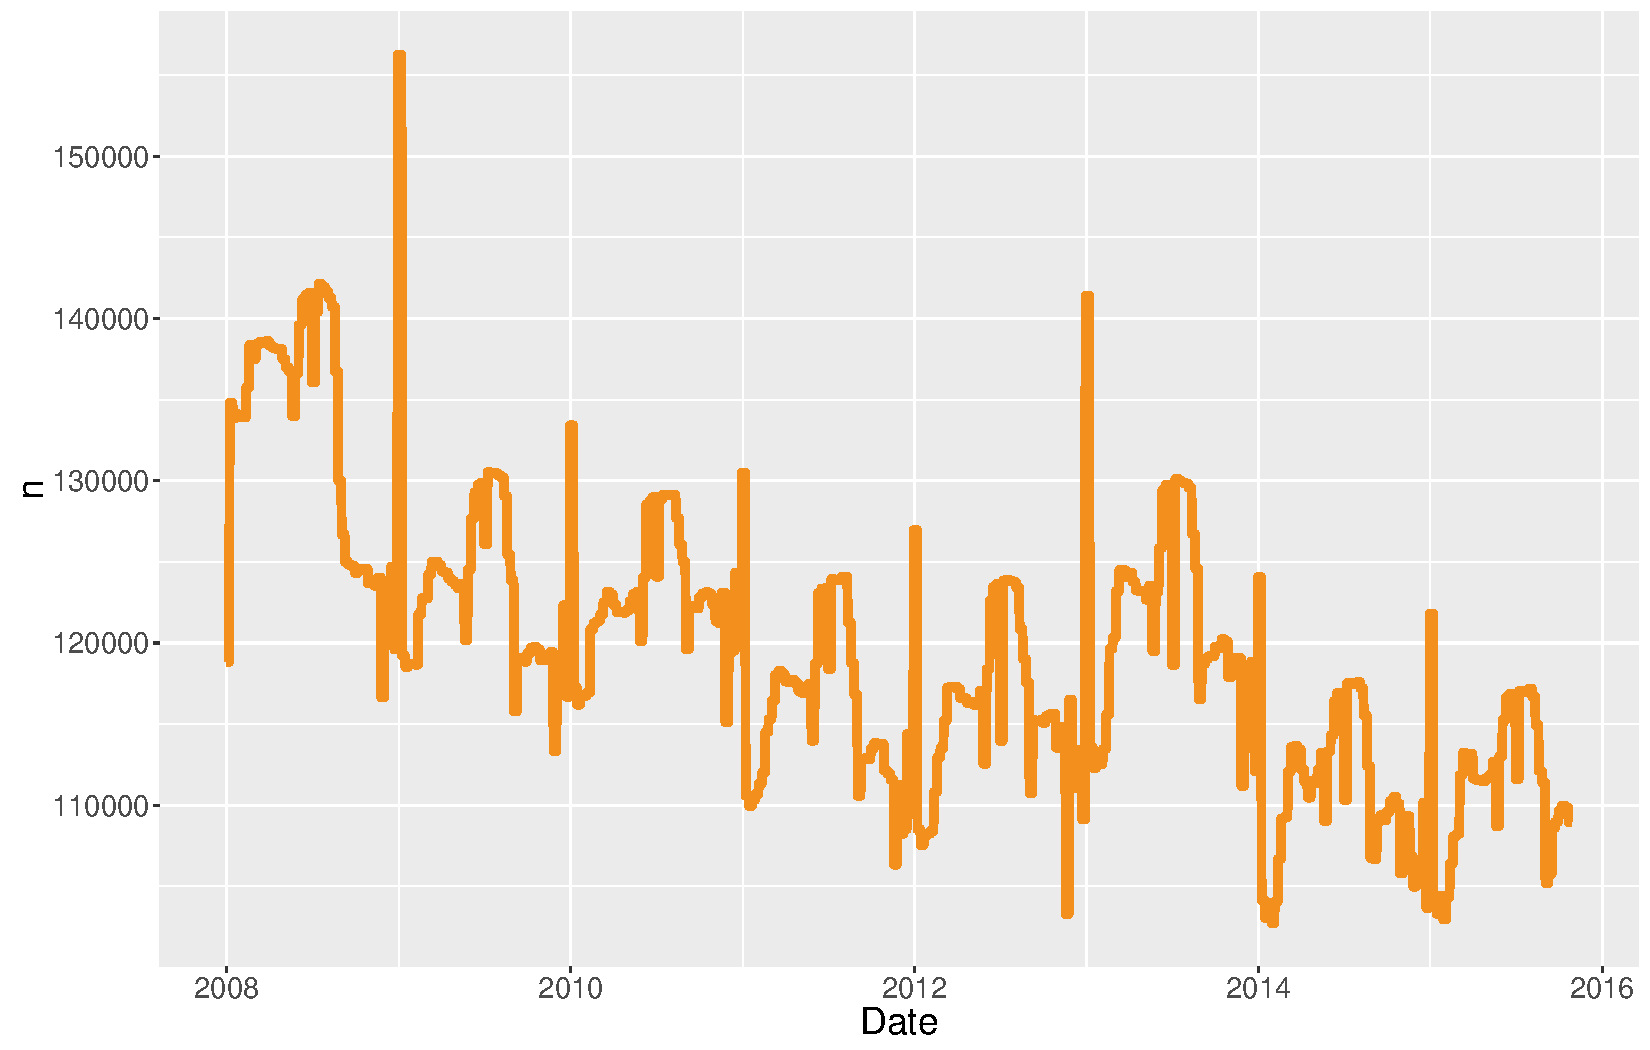
\includegraphics[width=\textwidth]{atlas-post-2008/Flights-by-week-1}
\end{figure*}

\begin{knitrout}
\definecolor{shadecolor}{rgb}{0.969, 0.969, 0.969}\color{fgcolor}\begin{kframe}
\begin{alltt}
\hlkwd{setkey}\hlstd{(unique_dates, Week)}
\hlstd{flights[,}\hlkwd{.}\hlstd{(}\hlkwc{n} \hlstd{= .N),} \hlkwc{keyby} \hlstd{= Week][unique_dates]}  \hlopt
  \hlkwd{distinct}\hlstd{(Week)} \hlopt
  \hlkwd{filter}\hlstd{(Week} \hlopt{<} \hlkwd{max}\hlstd{(Week))} \hlopt
  \hlkwd{mutate}\hlstd{(}\hlkwc{difference} \hlstd{= n} \hlopt{-} \hlkwd{lag}\hlstd{(n,} \hlnum{1}\hlstd{,} \hlkwc{default} \hlstd{=} \hlkwd{mean}\hlstd{(.}\hlopt{$}\hlstd{n)),}
         \hlkwc{Date} \hlstd{=} \hlkwd{fastPOSIXct}\hlstd{(}\hlkwd{paste0}\hlstd{(Year,} \hlstr{"-"}\hlstd{, Month,} \hlstr{"-"}\hlstd{, DayofMonth)),}
         \hlkwc{diff.lab} \hlstd{=} \hlkwd{ifelse}\hlstd{(}\hlkwd{ntile}\hlstd{(difference,} \hlnum{100}\hlstd{)} \hlopt{==} \hlnum{100}\hlstd{,}
                           \hlkwd{paste0}\hlstd{(Year,} \hlstr{"-"}\hlstd{, Month,} \hlstr{"-"}\hlstd{, DayofMonth),}
                           \hlnum{NA}\hlstd{))} \hlopt
  \hlkwd{ggplot}\hlstd{(}\hlkwd{aes}\hlstd{(}\hlkwc{x} \hlstd{= Date,} \hlkwc{y} \hlstd{= n))} \hlopt{+}
  \hlkwd{geom_line}\hlstd{(}\hlkwc{group} \hlstd{=} \hlnum{1}\hlstd{,} \hlkwc{size} \hlstd{=} \hlnum{2}\hlstd{)} \hlopt{+}
  \hlkwd{geom_point}\hlstd{()} \hlopt{+}
  \hlkwd{geom_text}\hlstd{(}\hlkwd{aes}\hlstd{(}\hlkwc{label} \hlstd{= diff.lab))} \hlopt{+}
  \hlkwd{scale_y_continuous}\hlstd{(}\hlkwc{label} \hlstd{= comma)}
\end{alltt}


{\ttfamily\noindent\color{warningcolor}{\#\# Warning: Removed 403 rows containing missing values (geom\_text).}}\end{kframe}
\end{knitrout}

\begin{knitrout}
\definecolor{shadecolor}{rgb}{0.969, 0.969, 0.969}\color{fgcolor}\begin{kframe}
\begin{alltt}
\hlstd{flights.by.week.and.carrier} \hlkwb{<-}
  \hlstd{flights[,}\hlkwd{.}\hlstd{(}\hlkwc{n} \hlstd{= .N),} \hlkwc{by} \hlstd{=} \hlkwd{list}\hlstd{(Week, UniqueCarrier)]}

\hlstd{biggest.carriers} \hlkwb{<-}
  \hlstd{flights[,}\hlkwd{.}\hlstd{(}\hlkwc{n} \hlstd{= .N),} \hlkwc{by} \hlstd{= UniqueCarrier][}\hlkwd{order}\hlstd{(}\hlopt{-}\hlstd{n)]} \hlopt
  \hlkwd{filter}\hlstd{(}\hlkwd{row_number}\hlstd{(}\hlopt{-}\hlstd{n)} \hlopt{<=} \hlnum{6}\hlstd{)} \hlopt
  \hlstd{UniqueCarrier}

\hlstd{nycflights.airlines[,Carrier_other} \hlkwb{:=} \hlkwd{ifelse}\hlstd{(UniqueCarrier} \hlopt \hlstd{biggest.carriers, UniqueCarrier,} \hlstr{"Other"}\hlstd{)]}

\hlstd{flights.by.week.and.carrier.other} \hlkwb{<-}
  \hlstd{flights.by.week.and.carrier} \hlopt
  \hlkwd{group_by}\hlstd{(Week,}
           \hlkwc{Carrier_other} \hlstd{=} \hlkwd{ifelse}\hlstd{(UniqueCarrier} \hlopt \hlstd{biggest.carriers, UniqueCarrier,} \hlstr{"Other"}\hlstd{))} \hlopt
  \hlkwd{summarise}\hlstd{(}\hlkwc{n} \hlstd{=} \hlkwd{sum}\hlstd{(n))} \hlopt
  \hlkwd{merge}\hlstd{(airlines,} \hlkwc{by.x} \hlstd{=} \hlstr{"Carrier_other"}\hlstd{,} \hlkwc{by.y} \hlstd{=} \hlstr{"carrier"}\hlstd{,} \hlkwc{all.x} \hlstd{=} \hlnum{TRUE}\hlstd{)} \hlopt
  \hlkwd{mutate}\hlstd{(}\hlkwc{Carrier_other} \hlstd{=} \hlkwd{factor}\hlstd{(Carrier_other,} \hlkwc{levels} \hlstd{=} \hlkwd{c}\hlstd{(biggest.carriers,} \hlstr{"Other"}\hlstd{)))}

\hlstd{flights.by.week.and.carrier.other} \hlopt
  \hlstd{convert_week_to_date} \hlopt
  \hlkwd{arrange}\hlstd{(Date, Carrier_other)} \hlopt
  \hlkwd{ggplot}\hlstd{(}\hlkwd{aes}\hlstd{(}\hlkwc{x} \hlstd{= Date,} \hlkwc{y} \hlstd{= n,} \hlkwc{fill} \hlstd{= Carrier_other))} \hlopt{+}
  \hlkwd{geom_area}\hlstd{()} \hlopt{+}
  \hlkwd{scale_y_continuous}\hlstd{(}\hlkwc{label} \hlstd{= scales}\hlopt{::}\hlstd{comma)} \hlopt{+}
  \hlkwd{scale_fill_brewer}\hlstd{(}\hlstr{""}\hlstd{,} \hlkwc{palette} \hlstd{=} \hlstr{"Spectral"}\hlstd{)} \hlopt{+}
  \hlkwd{guides}\hlstd{(}\hlkwc{fill} \hlstd{=} \hlkwd{guide_legend}\hlstd{(}\hlkwc{reverse} \hlstd{=} \hlnum{TRUE}\hlstd{))} \hlopt{+}
  \hlkwd{annotate}\hlstd{(}\hlstr{"blank"}\hlstd{,} \hlkwc{x} \hlstd{=} \hlkwd{fastPOSIXct}\hlstd{(}\hlstr{'2016-03-01'}\hlstd{),} \hlkwc{y} \hlstd{=} \hlnum{0}\hlstd{)} \hlopt{+}
  \hlkwd{scale_x_datetime}\hlstd{(}\hlkwc{expand} \hlstd{=} \hlkwd{c}\hlstd{(}\hlnum{0}\hlstd{,}\hlnum{0}\hlstd{))} \hlopt{+}
  \hlkwd{scale_y_continuous}\hlstd{(}\hlkwc{expand} \hlstd{=} \hlkwd{c}\hlstd{(}\hlnum{0}\hlstd{,}\hlnum{0}\hlstd{),} \hlkwc{label} \hlstd{= comma)} \hlopt{+}
  \hlkwd{theme}\hlstd{(}\hlkwc{legend.position} \hlstd{=} \hlstr{"right"}\hlstd{)}
\end{alltt}


{\ttfamily\noindent\itshape\color{messagecolor}{\#\# Scale for 'y' is already present. Adding another scale for 'y', which\\\#\# will replace the existing scale.}}\end{kframe}
\end{knitrout}
\begin{figure*}
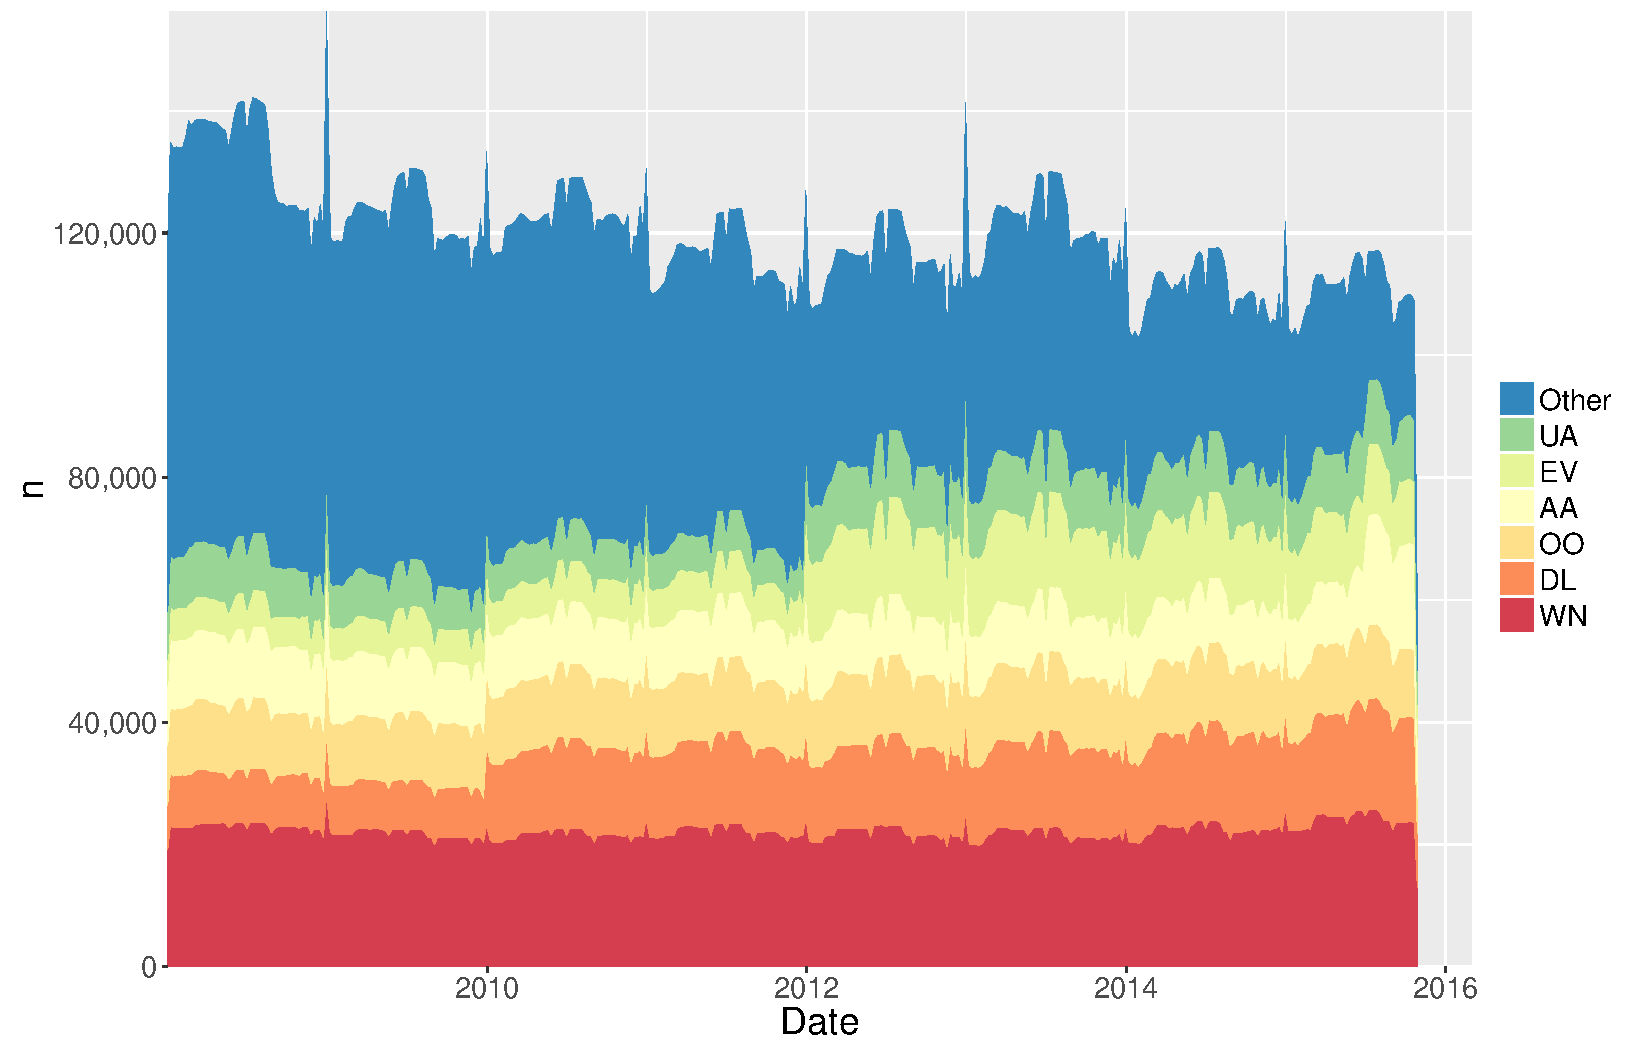
\includegraphics[width=\textwidth]{atlas-post-2008/Flights-by-week-and-carrier-1}
\end{figure*}

\begin{knitrout}
\definecolor{shadecolor}{rgb}{0.969, 0.969, 0.969}\color{fgcolor}\begin{kframe}
\begin{alltt}
\hlstd{flights.by.week.and.carrier.other} \hlopt
  \hlkwd{group_by}\hlstd{(Carrier_other)} \hlopt
  \hlkwd{mutate}\hlstd{(}\hlkwc{r} \hlstd{= n}\hlopt{/}\hlkwd{first}\hlstd{(n))} \hlopt
  \hlkwd{filter}\hlstd{(Week} \hlopt{<} \hlkwd{max}\hlstd{(Week))} \hlopt
  \hlkwd{mutate}\hlstd{(}\hlkwc{label.y} \hlstd{=} \hlkwd{ifelse}\hlstd{(Week} \hlopt{==} \hlkwd{max}\hlstd{(Week), r,} \hlnum{NA_real_}\hlstd{))} \hlopt
  \hlstd{convert_week_to_date} \hlopt
  \hlkwd{ggplot}\hlstd{(}\hlkwd{aes}\hlstd{(}\hlkwc{x} \hlstd{= Date,} \hlkwc{y} \hlstd{= r,} \hlkwc{color} \hlstd{= Carrier_other,} \hlkwc{group} \hlstd{= Carrier_other))} \hlopt{+}
  \hlkwd{geom_line}\hlstd{()} \hlopt{+}
  \hlkwd{geom_dl}\hlstd{(}\hlkwc{method} \hlstd{=} \hlstr{"last.qp"}\hlstd{,} \hlkwd{aes}\hlstd{(}\hlkwc{label} \hlstd{=} \hlkwd{ifelse}\hlstd{(}\hlkwd{is.na}\hlstd{(name),} \hlstr{"Other"}\hlstd{,} \hlkwd{gsub}\hlstd{(}\hlstr{"^([A-Za-z]+)\textbackslash{}\textbackslash{}b.*$"}\hlstd{,} \hlstr{"\textbackslash{}\textbackslash{}1"}\hlstd{,  name))))} \hlopt{+}
\hlcom{#   geom_text(aes(y = label.y, label = name}
\hlcom{#                 ), hjust = 0, nudge_x = 1) + }
  \hlcom{#scale_color_brewer(palette = "Spectral") +}
  \hlkwd{guides}\hlstd{(}\hlkwc{color} \hlstd{=} \hlkwd{guide_legend}\hlstd{(}\hlkwc{reverse} \hlstd{=} \hlnum{TRUE}\hlstd{))} \hlopt{+}
  \hlkwd{annotate}\hlstd{(}\hlstr{"blank"}\hlstd{,} \hlkwc{x} \hlstd{=} \hlkwd{fastPOSIXct}\hlstd{(}\hlstr{'2016-09-01'}\hlstd{),} \hlkwc{y} \hlstd{=} \hlnum{0}\hlstd{)} \hlopt{+}
  \hlkwd{scale_x_datetime}\hlstd{(}\hlkwc{expand} \hlstd{=} \hlkwd{c}\hlstd{(}\hlnum{0}\hlstd{,}\hlnum{0}\hlstd{))} \hlopt{+}
  \hlkwd{scale_y_continuous}\hlstd{(}\hlkwc{expand} \hlstd{=} \hlkwd{c}\hlstd{(}\hlnum{0}\hlstd{,}\hlnum{0}\hlstd{),} \hlkwc{label} \hlstd{= comma)} \hlopt{+}
  \hlkwd{theme}\hlstd{(}\hlkwc{legend.position} \hlstd{=} \hlstr{"none"}\hlstd{)}
\end{alltt}
\end{kframe}
\end{knitrout}

\begin{knitrout}
\definecolor{shadecolor}{rgb}{0.969, 0.969, 0.969}\color{fgcolor}\begin{kframe}
\begin{alltt}
\hlstd{cancellations.by.week} \hlkwb{<-}
  \hlstd{flights} \hlopt
  \hlkwd{select}\hlstd{(Week, Cancelled)} \hlopt
  \hlkwd{group_by}\hlstd{(Week)} \hlopt
  \hlkwd{summarise}\hlstd{(}\hlkwc{total_cancellations} \hlstd{=} \hlkwd{sum}\hlstd{(Cancelled))}

\hlstd{cancellations.by.week} \hlopt
  \hlstd{convert_week_to_date} \hlopt
  \hlkwd{ggplot}\hlstd{(}\hlkwd{aes}\hlstd{(}\hlkwc{x} \hlstd{= Date,} \hlkwc{y} \hlstd{= total_cancellations))} \hlopt{+}
  \hlkwd{geom_line}\hlstd{(}\hlkwc{group} \hlstd{=} \hlnum{1}\hlstd{)}
\end{alltt}
\end{kframe}
\end{knitrout}

\begin{knitrout}
\definecolor{shadecolor}{rgb}{0.969, 0.969, 0.969}\color{fgcolor}\begin{kframe}
\begin{alltt}
\hlstd{cancellations.by.month} \hlkwb{<-}
  \hlstd{flights} \hlopt
  \hlkwd{select}\hlstd{(Year, Month, Cancelled)} \hlopt
  \hlkwd{group_by}\hlstd{(Year, Month)} \hlopt
  \hlkwd{summarise}\hlstd{(}\hlkwc{total_cancellations} \hlstd{=} \hlkwd{sum}\hlstd{(Cancelled))}

\hlstd{cancellations.by.month} \hlopt
  \hlkwd{ggplot}\hlstd{(}\hlkwd{aes}\hlstd{(}\hlkwc{x} \hlstd{= Year} \hlopt{+} \hlstd{Month}\hlopt{/}\hlnum{12}\hlstd{,} \hlkwc{y} \hlstd{= total_cancellations))} \hlopt{+}
  \hlkwd{geom_line}\hlstd{()}
\end{alltt}
\end{kframe}
\end{knitrout}

\begin{knitrout}
\definecolor{shadecolor}{rgb}{0.969, 0.969, 0.969}\color{fgcolor}\begin{kframe}
\begin{alltt}
\hlstd{cancellations.by.year.carrier.other} \hlkwb{<-}
  \hlstd{flights} \hlopt
  \hlkwd{select}\hlstd{(Year, UniqueCarrier, Cancelled)} \hlopt
  \hlkwd{group_by}\hlstd{(Year, UniqueCarrier)} \hlopt
  \hlkwd{summarise}\hlstd{(}\hlkwc{total_cancellations} \hlstd{=} \hlkwd{sum}\hlstd{(Cancelled))} \hlopt
  \hlkwd{setkey}\hlstd{(UniqueCarrier)} \hlopt
  \hlstd{.[nycflights.airlines]} \hlopt
  \hlkwd{group_by}\hlstd{(Year, Carrier_other)} \hlopt
  \hlkwd{summarise}\hlstd{(}\hlkwc{total_cancellations} \hlstd{=} \hlkwd{sum}\hlstd{(total_cancellations))}

\hlstd{cancellations.by.year.carrier.other} \hlopt
  \hlkwd{mutate}\hlstd{(}\hlkwc{Carrier_other_f} \hlstd{=} \hlkwd{factor}\hlstd{(Carrier_other,} \hlkwc{levels} \hlstd{=} \hlkwd{c}\hlstd{(biggest.carriers,} \hlstr{"Other"}\hlstd{)))} \hlopt
  \hlkwd{arrange}\hlstd{(Year, Carrier_other_f)} \hlopt
  \hlkwd{ggplot}\hlstd{(}\hlkwd{aes}\hlstd{(}\hlkwc{x} \hlstd{= Year,} \hlkwc{y} \hlstd{= total_cancellations,} \hlkwc{fill} \hlstd{= Carrier_other_f))} \hlopt{+}
  \hlkwd{geom_area}\hlstd{()} \hlopt{+}
  \hlkwd{guides}\hlstd{(}\hlkwc{fill} \hlstd{=} \hlkwd{guide_legend}\hlstd{(}\hlkwc{reverse} \hlstd{=} \hlnum{TRUE}\hlstd{))} \hlopt{+}
  \hlkwd{scale_fill_brewer}\hlstd{(}\hlkwc{palette} \hlstd{=} \hlstr{"Spectral"}\hlstd{)}
\end{alltt}
\end{kframe}
\end{knitrout}

\begin{knitrout}
\definecolor{shadecolor}{rgb}{0.969, 0.969, 0.969}\color{fgcolor}\begin{kframe}
\begin{alltt}
\hlstd{expected.cancellations.by.month} \hlkwb{<-}
\hlcom{#   system.time(\{}
\hlcom{#   flights %>%}
\hlcom{#   select(Year, Month, UniqueCarrier, Cancelled) %>%}
\hlcom{#   group_by(Year, Month, Carrier_other = ifelse(UniqueCarrier %in% biggest.carriers, UniqueCarrier, "Other")) %>%}
\hlcom{#   summarise(expected_cancellation = mean(Cancelled))}
\hlcom{#   \})}
\hlcom{# system.time(\{}
\hlcom{#   flights[,Carrier_other := ifelse(UniqueCarrier %in% biggest.carriers, UniqueCarrier, "Other")] %>%}
\hlcom{#   .[,.(expected_cancellation = mean(Cancelled)), by = list(Year, Month, Carrier_other)]\})}

  \hlstd{flights} \hlopt
  \hlkwd{select}\hlstd{(Year, Month, UniqueCarrier, Cancelled)} \hlopt
  \hlcom{# Get Carrier_other variable}
    \hlkwd{setkey}\hlstd{(UniqueCarrier)} \hlopt
    \hlstd{.[nycflights.airlines]} \hlopt
  \hlkwd{group_by}\hlstd{(Year, Month, Carrier_other)} \hlopt
  \hlkwd{summarise}\hlstd{(}\hlkwc{expected_cancellation} \hlstd{=} \hlkwd{mean}\hlstd{(Cancelled))}


\hlstd{expected.cancellations.by.month} \hlopt
  \hlkwd{ggplot}\hlstd{(}\hlkwd{aes}\hlstd{(}\hlkwc{x} \hlstd{= Year} \hlopt{+} \hlstd{Month}\hlopt{/}\hlnum{12}\hlstd{,} \hlkwc{y} \hlstd{= expected_cancellation,} \hlkwc{group} \hlstd{= Carrier_other,} \hlkwc{color} \hlstd{= Carrier_other))} \hlopt{+}
  \hlkwd{geom_line}\hlstd{()}
\end{alltt}
\end{kframe}
\end{knitrout}

\begin{knitrout}
\definecolor{shadecolor}{rgb}{0.969, 0.969, 0.969}\color{fgcolor}\begin{kframe}
\begin{alltt}
\hlstd{expected.cancellations.by.week} \hlkwb{<-}
  \hlstd{flights} \hlopt
  \hlkwd{select}\hlstd{(Week, UniqueCarrier, Cancelled)} \hlopt
  \hlcom{# Get Carrier_other variable}
    \hlkwd{setkey}\hlstd{(UniqueCarrier)} \hlopt
    \hlstd{.[nycflights.airlines]} \hlopt
  \hlkwd{group_by}\hlstd{(Week, Carrier_other)} \hlopt
  \hlkwd{summarise}\hlstd{(}\hlkwc{expected_cancellation} \hlstd{=} \hlkwd{mean}\hlstd{(Cancelled))}

\hlstd{expected.cancellations.by.week} \hlopt
  \hlkwd{group_by}\hlstd{(Week)} \hlopt
  \hlkwd{mutate}\hlstd{(}\hlkwc{difference} \hlstd{= expected_cancellation} \hlopt{-} \hlkwd{mean}\hlstd{(expected_cancellation))} \hlopt
  \hlkwd{ggplot}\hlstd{(}\hlkwd{aes}\hlstd{(}\hlkwc{x} \hlstd{= Week,} \hlkwc{y} \hlstd{= difference))} \hlopt{+}
  \hlkwd{geom_area}\hlstd{(}\hlkwc{group} \hlstd{=} \hlnum{1}\hlstd{)} \hlopt{+}
  \hlkwd{facet_grid}\hlstd{(Carrier_other} \hlopt{~} \hlstd{.)}
\end{alltt}
\end{kframe}
\end{knitrout}

\begin{knitrout}
\definecolor{shadecolor}{rgb}{0.969, 0.969, 0.969}\color{fgcolor}\begin{kframe}
\begin{alltt}
\hlstd{expected.cancellations.by.month} \hlopt
  \hlkwd{group_by}\hlstd{(Year, Month)} \hlopt
  \hlkwd{mutate}\hlstd{(}\hlkwc{difference} \hlstd{= expected_cancellation} \hlopt{-} \hlkwd{mean}\hlstd{(expected_cancellation))} \hlopt
  \hlkwd{ggplot}\hlstd{(}\hlkwd{aes}\hlstd{(}\hlkwc{x} \hlstd{=} \hlkwd{as.Date}\hlstd{(}\hlkwd{paste0}\hlstd{(Year,} \hlstr{"-"}\hlstd{, Month,} \hlstr{"-01"}\hlstd{)),} \hlkwc{y} \hlstd{= difference))} \hlopt{+}
  \hlkwd{geom_area}\hlstd{(}\hlkwc{group} \hlstd{=} \hlnum{1}\hlstd{)} \hlopt{+}
  \hlkwd{facet_grid}\hlstd{(Carrier_other} \hlopt{~} \hlstd{.)} \hlopt{+}
  \hlkwd{theme}\hlstd{(}\hlkwc{axis.title} \hlstd{=} \hlkwd{element_blank}\hlstd{())}
\end{alltt}
\end{kframe}
\end{knitrout}
\begin{figure*}
\caption{Southwest airlines (and Delta Air Lines from the start of 2011) have had consistently lower cancellation rates. ExpressJet has had substantially higher.}
\vspace*{11pt}
\caption*{The difference of each airline's expected cancellation (cancellations per flight) from the average expected cancellation across all airlines, monthly.}
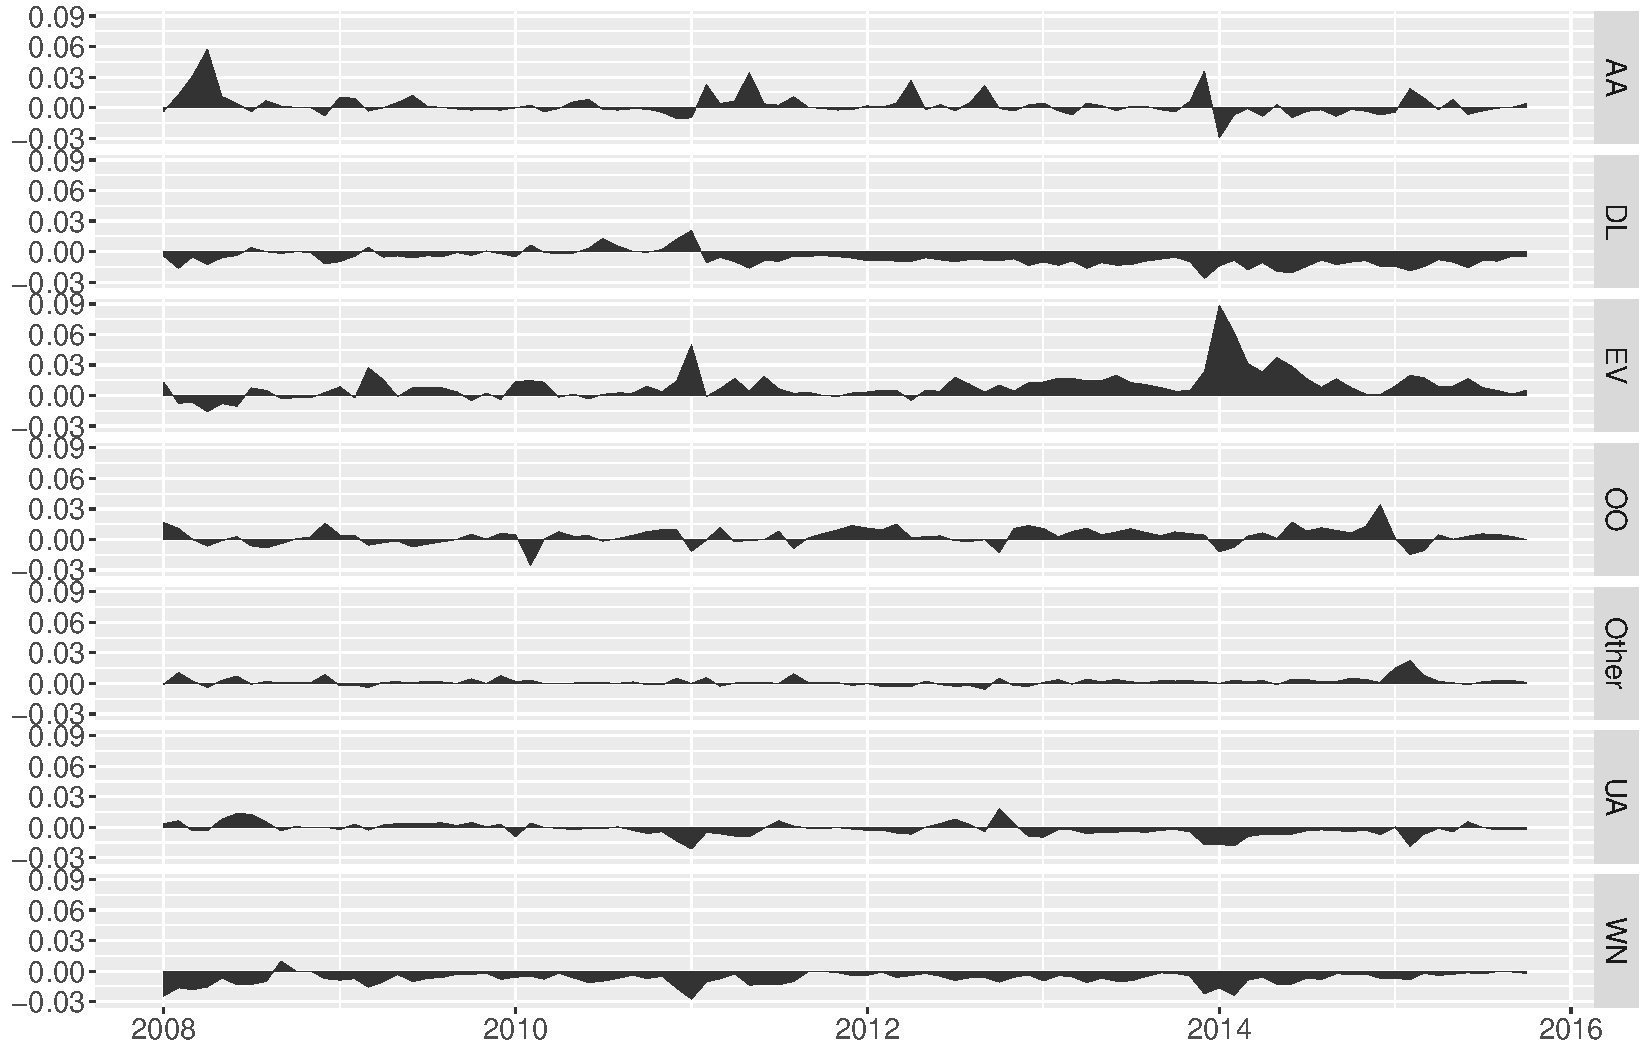
\includegraphics[width=2\columnwidth]{atlas-post-2008/Expected-cancellation-by-month-difference-1}
\end{figure*}

\begin{knitrout}
\definecolor{shadecolor}{rgb}{0.969, 0.969, 0.969}\color{fgcolor}\begin{kframe}
\begin{alltt}
\hlstd{ArrDelays.by.week} \hlkwb{<-}
  \hlstd{flights} \hlopt
  \hlkwd{select}\hlstd{(Week, ArrDelay)} \hlopt
  \hlkwd{group_by}\hlstd{(Week)} \hlopt
  \hlkwd{summarise}\hlstd{(}\hlkwc{total_ArrDelay} \hlstd{=} \hlkwd{sum}\hlstd{(ArrDelay,} \hlkwc{na.rm} \hlstd{=} \hlnum{TRUE}\hlstd{))}

\hlstd{ArrDelays.by.week} \hlopt
  \hlkwd{ggplot}\hlstd{(}\hlkwd{aes}\hlstd{(Week, total_ArrDelay))} \hlopt{+}
  \hlkwd{geom_area}\hlstd{(}\hlkwc{group} \hlstd{=} \hlnum{1}\hlstd{)} \hlopt{+}
  \hlkwd{geom_hline}\hlstd{(}\hlkwc{yintercept} \hlstd{=} \hlnum{0}\hlstd{,} \hlkwc{color} \hlstd{=} \hlstr{"black"}\hlstd{)}
\end{alltt}
\end{kframe}
\end{knitrout}

\begin{knitrout}
\definecolor{shadecolor}{rgb}{0.969, 0.969, 0.969}\color{fgcolor}\begin{kframe}
\begin{alltt}
\hlstd{ArrDelays.by.month} \hlkwb{<-}
  \hlstd{flights} \hlopt
  \hlkwd{select}\hlstd{(Year, Month, ArrDelay)} \hlopt
  \hlkwd{group_by}\hlstd{(Year, Month)} \hlopt
  \hlkwd{summarise}\hlstd{(}\hlkwc{total_ArrDelay} \hlstd{=} \hlkwd{sum}\hlstd{(ArrDelay,} \hlkwc{na.rm} \hlstd{=} \hlnum{TRUE}\hlstd{))}

\hlstd{ArrDelays.by.month} \hlopt
  \hlkwd{ggplot}\hlstd{(}\hlkwd{aes}\hlstd{(}\hlkwd{as.Date}\hlstd{(}\hlkwd{sprintf}\hlstd{(}\hlstr{"%d-%02d-01"}\hlstd{, Year, Month)), total_ArrDelay))} \hlopt{+}
  \hlkwd{geom_area}\hlstd{(}\hlkwc{group} \hlstd{=} \hlnum{1}\hlstd{)} \hlopt{+}
  \hlkwd{geom_hline}\hlstd{(}\hlkwc{yintercept} \hlstd{=} \hlnum{0}\hlstd{,} \hlkwc{color} \hlstd{=} \hlstr{"black"}\hlstd{)}
\end{alltt}
\end{kframe}
\end{knitrout}

\begin{knitrout}
\definecolor{shadecolor}{rgb}{0.969, 0.969, 0.969}\color{fgcolor}\begin{kframe}
\begin{alltt}
\hlstd{ArrDelays.by.month} \hlopt
  \hlstd{ungroup} \hlopt
  \hlkwd{mutate}\hlstd{(}\hlkwc{rel_delay} \hlstd{= total_ArrDelay}\hlopt{/}\hlkwd{mean}\hlstd{(total_ArrDelay))}

\hlstd{cancellations.by.month} \hlopt
  \hlstd{ungroup} \hlopt
  \hlkwd{mutate}\hlstd{(}\hlkwc{rel_cancellations} \hlstd{= total_cancellations} \hlopt{/} \hlkwd{mean}\hlstd{(total_cancellations))}

\hlkwd{setkey}\hlstd{(ArrDelays.by.month, Year, Month)}
\hlkwd{setkey}\hlstd{(cancellations.by.month, Year, Month)}
\hlstd{ArrDelays.by.month[cancellations.by.month]} \hlopt
  \hlkwd{select}\hlstd{(Year, Month,} \hlkwd{starts_with}\hlstd{(}\hlstr{"rel"}\hlstd{))} \hlopt
  \hlkwd{melt.data.table}\hlstd{(}\hlkwc{measure.vars} \hlstd{=} \hlkwd{c}\hlstd{(}\hlstr{"rel_delay"}\hlstd{,} \hlstr{"rel_cancellations"}\hlstd{),} \hlkwc{variable.name} \hlstd{=} \hlstr{"delay_or_cancel"}\hlstd{)} \hlopt
  \hlkwd{ggplot}\hlstd{(}\hlkwd{aes}\hlstd{(}\hlkwd{as.Date}\hlstd{(}\hlkwd{sprintf}\hlstd{(}\hlstr{"%d-%02d-01"}\hlstd{, Year, Month)), value,} \hlkwc{fill} \hlstd{= delay_or_cancel))} \hlopt{+}
  \hlkwd{geom_bar}\hlstd{(}\hlkwc{stat} \hlstd{=} \hlstr{"identity"}\hlstd{,} \hlkwc{position} \hlstd{=} \hlstr{"stack"}\hlstd{,} \hlkwc{width} \hlstd{=} \hlnum{30}\hlstd{)} \hlopt{+}
  \hlkwd{theme}\hlstd{(}\hlkwc{legend.position} \hlstd{=} \hlstr{"top"}\hlstd{)}
\end{alltt}


{\ttfamily\noindent\color{warningcolor}{\#\# Warning: Stacking not well defined when ymin != 0}}

{\ttfamily\noindent\color{warningcolor}{\#\# Warning: position\_stack requires non-overlapping x intervals}}\end{kframe}
\end{knitrout}




\section{Which airport causes the most delays}
\begin{knitrout}
\definecolor{shadecolor}{rgb}{0.969, 0.969, 0.969}\color{fgcolor}\begin{kframe}
\begin{alltt}
\hlcom{# system.time(\{}
\hlcom{# flights.by.origin <- }
\hlcom{#   count(flights, Origin) %>%}
\hlcom{#   arrange(desc(n))}
\hlcom{# \})}
\hlcom{# 8 s.}

\hlstd{flights.by.origin} \hlkwb{<-}
    \hlstd{flights[,}\hlkwd{.}\hlstd{(}\hlkwc{n} \hlstd{= .N),} \hlkwc{by} \hlstd{= Origin][}\hlkwd{order}\hlstd{(}\hlopt{-}\hlstd{n)]}
\hlcom{# 0.27s}

\hlstd{flights.by.airport.carrier} \hlkwb{<-}
\hlcom{#   flights %>%}
\hlcom{#   count(Origin, UniqueCarrier) %>%}
\hlcom{#   arrange(desc(n))}
  \hlstd{flights[,}\hlkwd{.}\hlstd{(}\hlkwc{n} \hlstd{= .N),} \hlkwc{by} \hlstd{=} \hlkwd{list}\hlstd{(Origin, UniqueCarrier)][}\hlkwd{order}\hlstd{(}\hlopt{-}\hlstd{n)]}

\hlstd{hubs} \hlkwb{<-}
  \hlstd{flights.by.airport.carrier} \hlopt
  \hlkwd{group_by}\hlstd{(UniqueCarrier)} \hlopt
  \hlkwd{filter}\hlstd{(n} \hlopt{>=} \hlkwd{nth}\hlstd{(n,} \hlkwc{order_by} \hlstd{=} \hlopt{-}\hlnum{1}\hlopt{*}\hlstd{n,} \hlnum{2}\hlstd{))}

\hlstd{hub1.by.carrier} \hlkwb{<-}
  \hlstd{hubs} \hlopt
  \hlkwd{group_by}\hlstd{(UniqueCarrier)} \hlopt
  \hlkwd{filter}\hlstd{(n} \hlopt{==} \hlkwd{max}\hlstd{(n))} \hlopt
  \hlkwd{select}\hlstd{(}\hlopt{-}\hlstd{n)} \hlopt
  \hlkwd{setnames}\hlstd{(}\hlstr{"Origin"}\hlstd{,} \hlstr{"Hub1"}\hlstd{)} \hlopt
  \hlkwd{setkey}\hlstd{(UniqueCarrier)}

\hlstd{hub2.by.carrier} \hlkwb{<-}
  \hlstd{hubs} \hlopt
  \hlkwd{group_by}\hlstd{(UniqueCarrier)} \hlopt
  \hlkwd{filter}\hlstd{(n} \hlopt{!=} \hlkwd{max}\hlstd{(n))} \hlopt
  \hlkwd{select}\hlstd{(}\hlopt{-}\hlstd{n)} \hlopt
  \hlkwd{setnames}\hlstd{(}\hlstr{"Origin"}\hlstd{,} \hlstr{"Hub2"}\hlstd{)} \hlopt
  \hlkwd{setkey}\hlstd{(UniqueCarrier)}
\end{alltt}
\end{kframe}
\end{knitrout}

\begin{knitrout}
\definecolor{shadecolor}{rgb}{0.969, 0.969, 0.969}\color{fgcolor}\begin{kframe}
\begin{alltt}
\hlcom{# Define hubbiness to be the Gini coefficient of each carrier.}
\hlstd{hubbiness.by.carrier} \hlkwb{<-}
  \hlstd{flights} \hlopt
  \hlkwd{select}\hlstd{(UniqueCarrier, Origin)} \hlopt
  \hlkwd{group_by}\hlstd{(UniqueCarrier, Origin)} \hlopt
  \hlkwd{tally}\hlstd{()} \hlopt
  \hlstd{ungroup} \hlopt
  \hlkwd{group_by}\hlstd{(UniqueCarrier)} \hlopt
  \hlkwd{summarise}\hlstd{(}\hlkwc{gini} \hlstd{= ineq}\hlopt{::}\hlkwd{Gini}\hlstd{(n))}

\hlstd{hubbiness.by.carrier} \hlopt
  \hlstd{ungroup} \hlopt
  \hlkwd{setkey}\hlstd{(UniqueCarrier)} \hlopt
  \hlkwd{merge}\hlstd{(nycflights.airlines)} \hlopt
  \hlstd{ungroup} \hlopt
  \hlkwd{arrange}\hlstd{(}\hlkwd{desc}\hlstd{(gini))} \hlopt
  \hlkwd{mutate}\hlstd{(}\hlkwc{short_name} \hlstd{=} \hlkwd{factor}\hlstd{(short_name,} \hlkwc{levels} \hlstd{= .}\hlopt{$}\hlstd{short_name))} \hlopt
  \hlstd{\{}
    \hlkwd{ggplot}\hlstd{(.,} \hlkwd{aes}\hlstd{(}\hlkwc{x} \hlstd{= short_name,} \hlkwc{y} \hlstd{= gini,} \hlkwc{order} \hlstd{= gini))} \hlopt{+}
      \hlkwd{geom_bar}\hlstd{(}\hlkwc{stat} \hlstd{=} \hlstr{"identity"}\hlstd{,} \hlkwc{width} \hlstd{=} \hlnum{0.9}\hlstd{)} \hlopt{+}
      \hlkwd{coord_flip}\hlstd{()} \hlopt{+}
      \hlkwd{geom_text}\hlstd{(}\hlkwd{aes}\hlstd{(}\hlkwc{label} \hlstd{=} \hlkwd{paste}\hlstd{(short_name,} \hlkwd{percent}\hlstd{(gini))),} \hlkwc{hjust} \hlstd{=} \hlnum{0}\hlstd{,} \hlkwc{nudge_y} \hlstd{=} \hlnum{0.025}\hlstd{)} \hlopt{+}
      \hlkwd{theme}\hlstd{(}\hlkwc{axis.title.y} \hlstd{=} \hlkwd{element_blank}\hlstd{(),} \hlkwc{axis.text.y} \hlstd{=} \hlkwd{element_blank}\hlstd{())} \hlopt{+}
      \hlkwd{scale_y_continuous}\hlstd{(}\hlstr{"Gini of airport volume"}\hlstd{,} \hlkwc{expand} \hlstd{=} \hlkwd{c}\hlstd{(}\hlnum{0}\hlstd{,}\hlnum{0}\hlstd{),} \hlkwc{limits} \hlstd{=} \hlkwd{c}\hlstd{(}\hlnum{0}\hlstd{,} \hlkwd{max}\hlstd{(.}\hlopt{$}\hlstd{gini)} \hlopt{*} \hlnum{1.3}\hlstd{),} \hlkwc{label} \hlstd{= percent)}
  \hlstd{\}}
\end{alltt}
\end{kframe}
\end{knitrout}
\begin{figure}
\makebox[\textwidth][l]{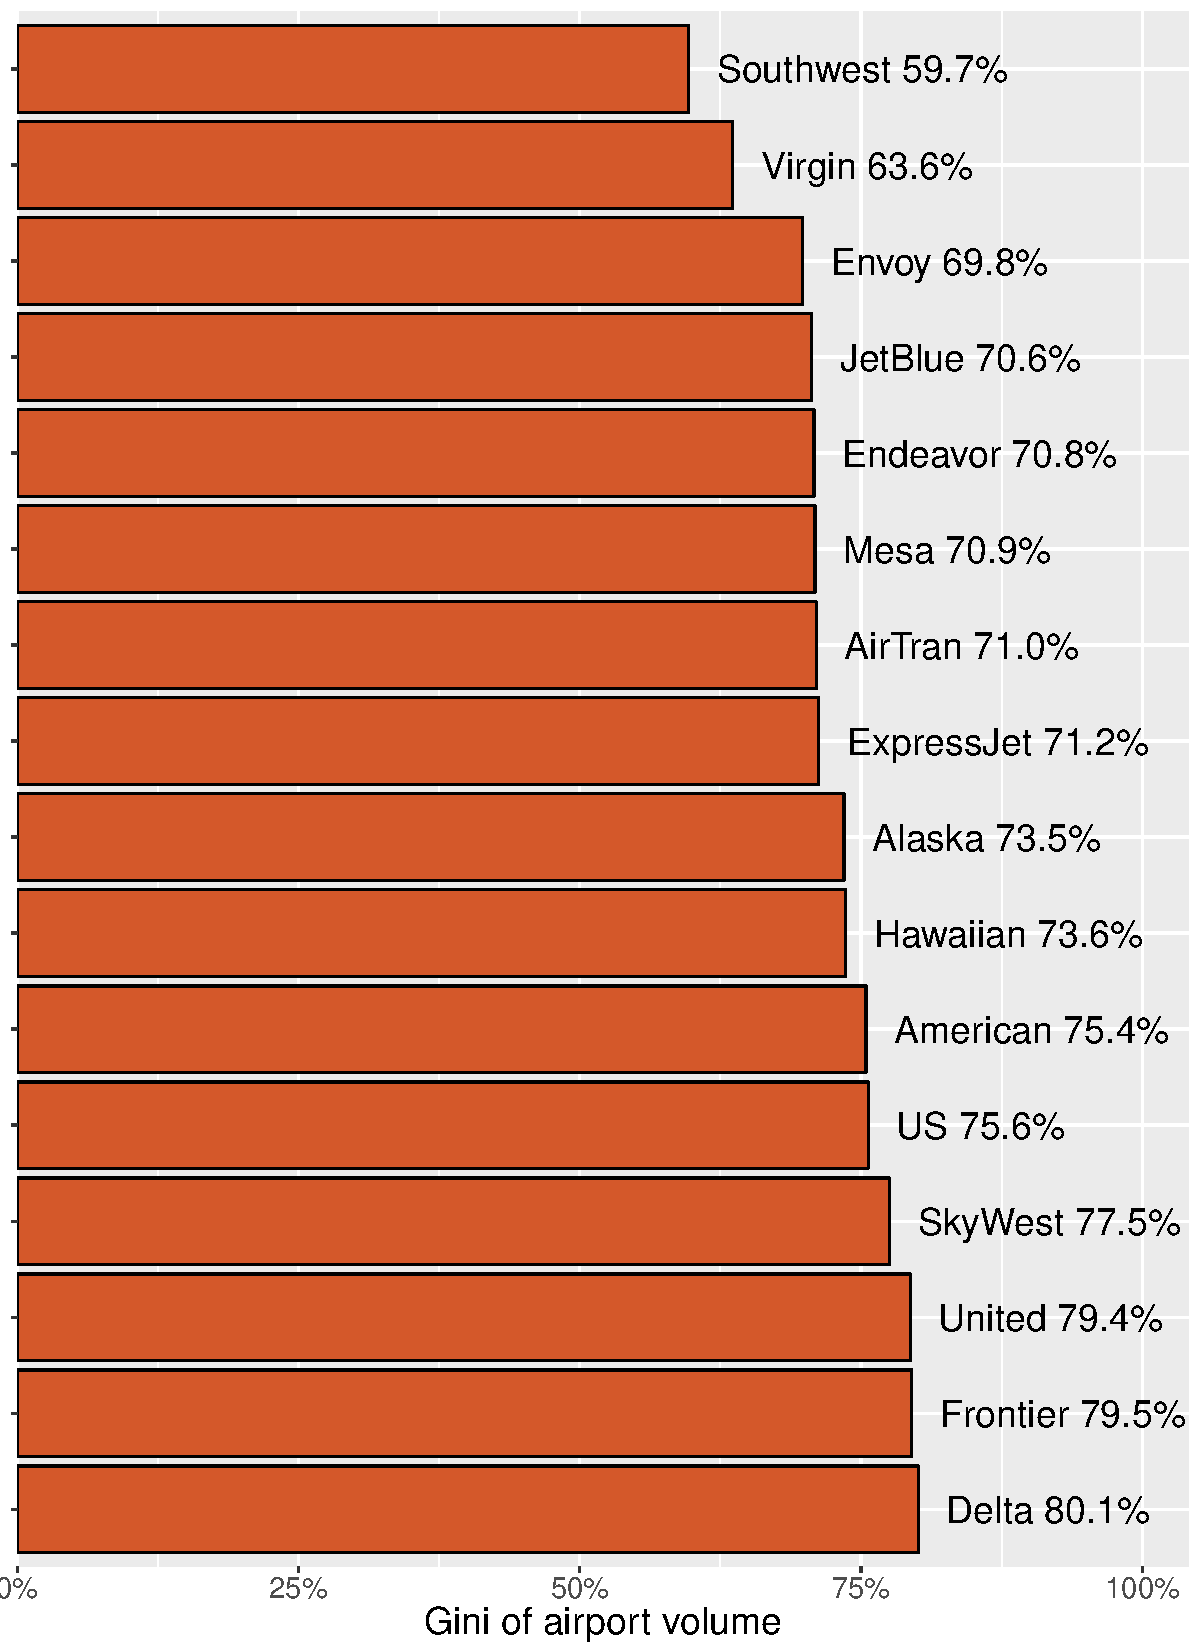
\includegraphics[width=1.5\columnwidth]{atlas-post-2008/Hubbiness-1}}
\end{figure}

\begin{knitrout}
\definecolor{shadecolor}{rgb}{0.969, 0.969, 0.969}\color{fgcolor}\begin{kframe}
\begin{alltt}
\hlkwd{ggplot}\hlstd{(hubbiness.by.carrier[flights.by.carrier][nycflights.airlines],}
       \hlkwd{aes}\hlstd{(}\hlkwc{x} \hlstd{= gini,} \hlkwc{y} \hlstd{= n))} \hlopt{+}
  \hlkwd{geom_point}\hlstd{(}\hlkwc{size} \hlstd{=} \hlnum{2}\hlstd{)} \hlopt{+}
  \hlkwd{geom_text_repel}\hlstd{(}\hlkwd{aes}\hlstd{(}\hlkwc{label} \hlstd{= short_name),} \hlkwc{fontface} \hlstd{=} \hlstr{"bold"}\hlstd{,} \hlkwc{size} \hlstd{=} \hlnum{6}\hlstd{)} \hlopt{+}
  \hlkwd{scale_y_continuous}\hlstd{(}\hlstr{"Volume (2008-2015)"}\hlstd{,} \hlkwc{labels} \hlstd{=} \hlkwa{function}\hlstd{(}\hlkwc{x}\hlstd{)}\hlkwd{paste0}\hlstd{(x}\hlopt{/}\hlnum{1e6}\hlstd{,} \hlstr{"M"}\hlstd{))}
\end{alltt}


{\ttfamily\noindent\bfseries\color{errorcolor}{\#\# Error in `[.data.table`(hubbiness.by.carrier[flights.by.carrier], nycflights.airlines): When i is a data.table (or character vector), x must be keyed (i.e. sorted, and, marked as sorted) so data.table knows which columns to join to and take advantage of x being sorted. Call setkey(x,...) first, see ?setkey.}}\end{kframe}
\end{knitrout}

\begin{knitrout}
\definecolor{shadecolor}{rgb}{0.969, 0.969, 0.969}\color{fgcolor}\begin{kframe}
\begin{alltt}
\hlstd{flights.by.carrier.year} \hlkwb{<-}
  \hlstd{flights[,}\hlkwd{.}\hlstd{(}\hlkwc{n} \hlstd{= .N),} \hlkwc{by} \hlstd{=} \hlkwd{list}\hlstd{(Year, UniqueCarrier)]}
\hlkwd{setkey}\hlstd{(flights.by.carrier.year, Year, UniqueCarrier)}
\hlstd{hubbiness.by.carrier.year} \hlkwb{<-}
  \hlstd{flights} \hlopt
  \hlkwd{select}\hlstd{(Year, UniqueCarrier, Origin)} \hlopt
  \hlkwd{count}\hlstd{(Year, UniqueCarrier, Origin)} \hlopt
  \hlkwd{group_by}\hlstd{(Year, UniqueCarrier)} \hlopt
  \hlkwd{summarise}\hlstd{(}\hlkwc{gini} \hlstd{= ineq}\hlopt{::}\hlkwd{Gini}\hlstd{(n))} \hlopt
  \hlkwd{setkey}\hlstd{(Year, UniqueCarrier)}

\hlkwd{setkey}\hlstd{(hubbiness.by.carrier.year, Year, UniqueCarrier)}
\hlkwd{merge}\hlstd{(hubbiness.by.carrier.year[flights.by.carrier.year], nycflights.airlines,} \hlkwc{by} \hlstd{=} \hlstr{"UniqueCarrier"}\hlstd{)} \hlopt
  \hlkwd{filter}\hlstd{(UniqueCarrier} \hlopt \hlkwd{select_large_carriers}\hlstd{(}\hlnum{9}\hlstd{))} \hlopt
  \hlkwd{mutate}\hlstd{(}\hlkwc{tempCarrierGroup} \hlstd{=} \hlkwd{factor}\hlstd{(}\hlkwd{ifelse}\hlstd{(UniqueCarrier} \hlopt{==} \hlstr{"WN"}\hlstd{,}
                                          \hlnum{1}\hlstd{,}
                                          \hlkwd{ifelse}\hlstd{(UniqueCarrier} \hlopt \hlkwd{select_large_carriers}\hlstd{(}\hlnum{5}\hlstd{),}
                                                 \hlnum{2}\hlstd{,}
                                                 \hlnum{3}\hlstd{))))} \hlopt
  \hlkwd{ggplot}\hlstd{(.,}
       \hlkwd{aes}\hlstd{(}\hlkwc{x} \hlstd{= gini,} \hlkwc{y} \hlstd{= n))} \hlopt{+}
  \hlkwd{geom_point}\hlstd{(}\hlkwd{aes}\hlstd{(}\hlkwc{alpha} \hlstd{= Year,} \hlkwc{color} \hlstd{= UniqueCarrier),} \hlkwc{size} \hlstd{=} \hlnum{4}\hlstd{)} \hlopt{+}
  \hlkwd{geom_line}\hlstd{(}\hlkwd{aes}\hlstd{(}\hlkwc{group} \hlstd{= UniqueCarrier,} \hlkwc{color} \hlstd{= UniqueCarrier),} \hlkwc{size} \hlstd{=} \hlnum{1}\hlstd{)} \hlopt{+}
  \hlkwd{scale_color_manual}\hlstd{(}\hlkwc{values} \hlstd{= carrier.colors)} \hlopt{+}
  \hlcom{#facet_grid(tempCarrierGroup~.) + }
  \hlkwd{geom_text_repel}\hlstd{(}\hlkwd{aes}\hlstd{(}\hlkwc{label} \hlstd{=} \hlkwd{ifelse}\hlstd{(Year} \hlopt{==} \hlkwd{max}\hlstd{(Year), short_name,} \hlnum{NA_character_}\hlstd{),}
                      \hlkwc{color} \hlstd{= UniqueCarrier),}
                  \hlkwc{fontface} \hlstd{=} \hlstr{"bold"}\hlstd{,} \hlkwc{size} \hlstd{=} \hlnum{6}\hlstd{)} \hlopt{+}
  \hlkwd{scale_y_continuous}\hlstd{(}\hlstr{"Volume"}\hlstd{,} \hlkwc{labels} \hlstd{=} \hlkwa{function}\hlstd{(}\hlkwc{x}\hlstd{)}\hlkwd{paste0}\hlstd{(x}\hlopt{/}\hlnum{1e6}\hlstd{,} \hlstr{"M"}\hlstd{))} \hlopt{+}
  \hlkwd{theme_dark}\hlstd{()} \hlopt{+}
  \hlkwd{theme}\hlstd{(}\hlkwc{legend.position} \hlstd{=} \hlstr{"none"}\hlstd{)}
\end{alltt}


{\ttfamily\noindent\color{warningcolor}{\#\# Warning: Removed 63 rows containing missing values (geom\_text\_repel).}}\end{kframe}
\end{knitrout}

\begin{knitrout}
\definecolor{shadecolor}{rgb}{0.969, 0.969, 0.969}\color{fgcolor}\begin{kframe}
\begin{alltt}
\hlstd{cancelled.flights.with.hub.cancelled} \hlkwb{<-}
  \hlstd{flights} \hlopt
  \hlkwd{select}\hlstd{(UniqueCarrier, Origin, Year, Month, DayofMonth, Cancelled)} \hlopt
  \hlkwd{setkey}\hlstd{(UniqueCarrier)} \hlopt
  \hlstd{data.table}\hlopt{:::}\hlkwd{merge.data.table}\hlstd{(hub1.by.carrier)} \hlopt
  \hlstd{data.table}\hlopt{:::}\hlkwd{merge.data.table}\hlstd{(hub2.by.carrier)}  \hlopt
  \hlkwd{group_by}\hlstd{(UniqueCarrier, Year, Month, DayofMonth)} \hlopt
  \hlkwd{summarise}\hlstd{(}\hlkwc{total_cancellations} \hlstd{=} \hlkwd{sum}\hlstd{(Cancelled),}
            \hlkwc{cancelled_at_hub1} \hlstd{=} \hlkwd{sum}\hlstd{(Cancelled} \hlopt{*} \hlstd{(Origin} \hlopt{==} \hlstd{Hub1)),}
            \hlkwc{cancelled_at_hub2} \hlstd{=} \hlkwd{sum}\hlstd{(Cancelled} \hlopt{*} \hlstd{(Origin} \hlopt{==} \hlstd{Hub2)))}
\end{alltt}
\end{kframe}
\end{knitrout}

\begin{knitrout}
\definecolor{shadecolor}{rgb}{0.969, 0.969, 0.969}\color{fgcolor}\begin{kframe}
\begin{alltt}
\hlstd{cancelled.flights.with.hub.cancelled} \hlopt
  \hlkwd{filter}\hlstd{(UniqueCarrier} \hlopt \hlstd{biggest.carriers)} \hlopt
  \hlkwd{ggplot}\hlstd{(}\hlkwd{aes}\hlstd{(}\hlkwc{x} \hlstd{= cancelled_at_hub1,} \hlkwc{y} \hlstd{= total_cancellations} \hlopt{-} \hlstd{cancelled_at_hub1))} \hlopt{+}
  \hlkwd{geom_point}\hlstd{(}\hlkwd{aes}\hlstd{(}\hlkwc{color} \hlstd{= UniqueCarrier))} \hlopt{+}
  \hlkwd{scale_color_brewer}\hlstd{(}\hlkwc{palette} \hlstd{=} \hlstr{"Spectral"}\hlstd{)} \hlopt{+}
  \hlkwd{guides}\hlstd{(}\hlkwc{color} \hlstd{=} \hlnum{FALSE}\hlstd{)} \hlopt{+}
  \hlkwd{facet_wrap}\hlstd{(}\hlopt{~}\hlstd{UniqueCarrier)} \hlopt{+}
  \hlkwd{theme_dark}\hlstd{()}
\end{alltt}
\end{kframe}
\end{knitrout}
\begin{figure*}
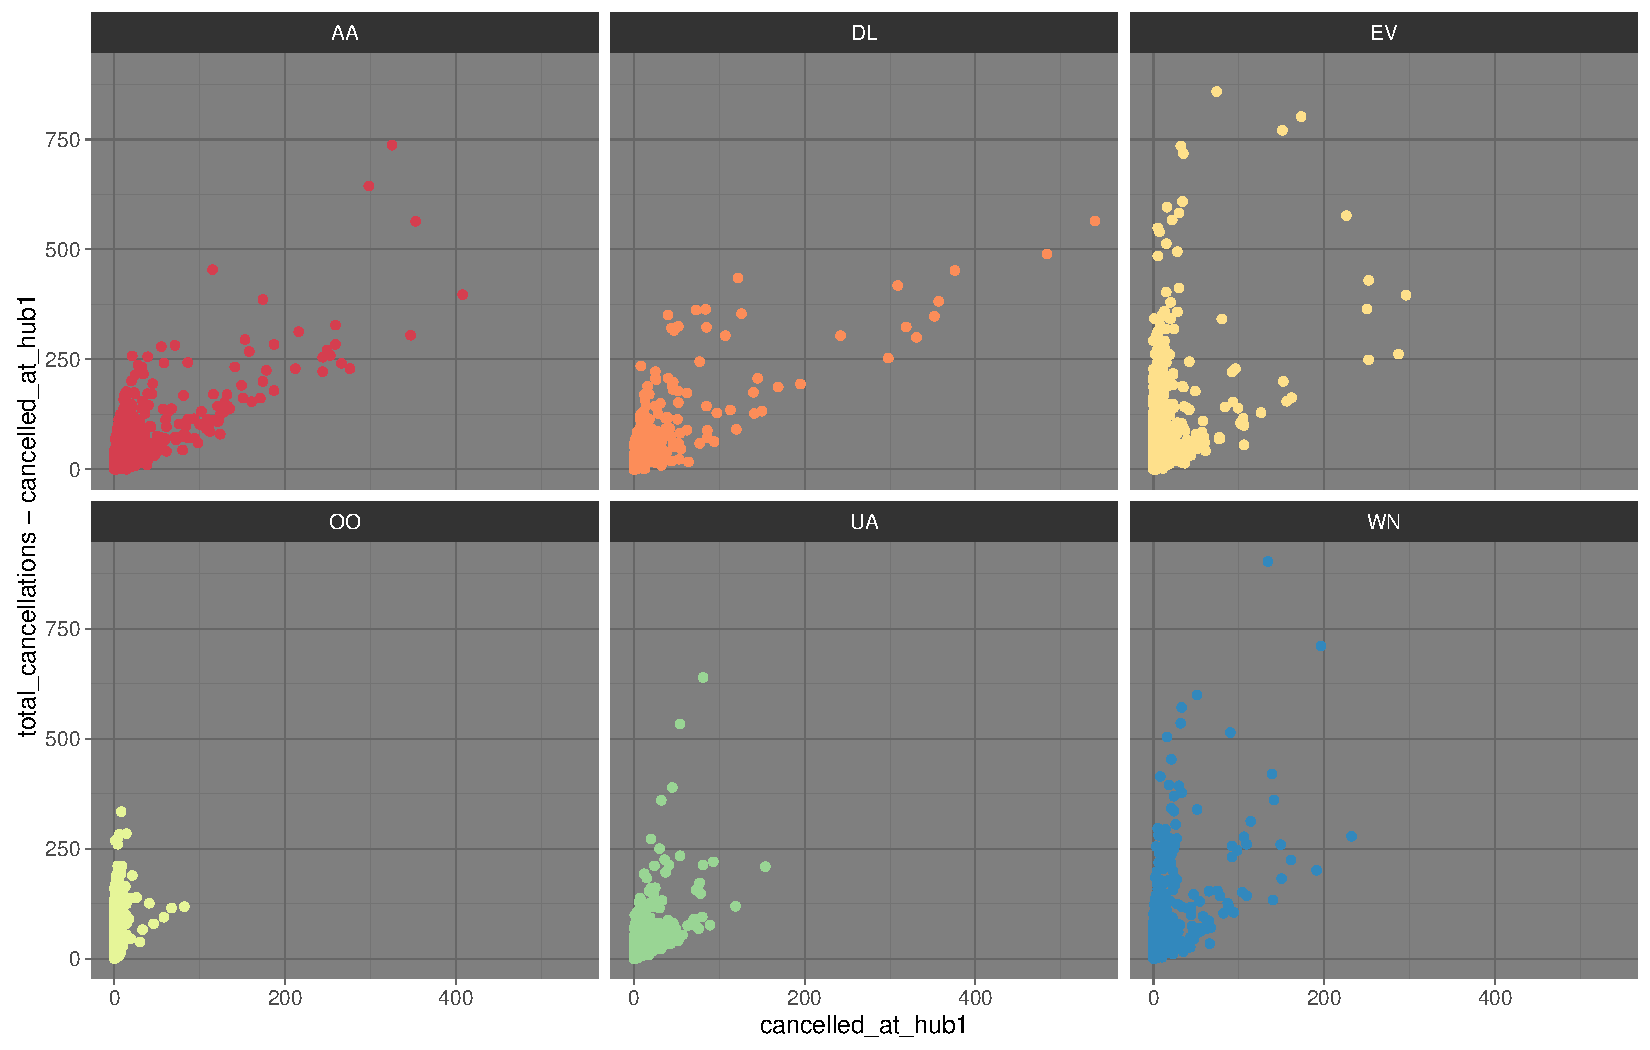
\includegraphics[width=\textwidth]{atlas-post-2008/cancelled-relative-hub1-plot-1}
\end{figure*}


\begin{knitrout}
\definecolor{shadecolor}{rgb}{0.969, 0.969, 0.969}\color{fgcolor}\begin{kframe}
\begin{alltt}
\hlstd{cancelled.flights.with.hub.cancelled} \hlopt
  \hlkwd{filter}\hlstd{(UniqueCarrier} \hlopt \hlstd{biggest.carriers)} \hlopt
  \hlkwd{ggplot}\hlstd{(}\hlkwd{aes}\hlstd{(}\hlkwc{x} \hlstd{= cancelled_at_hub1,} \hlkwc{y} \hlstd{= total_cancellations} \hlopt{-} \hlstd{cancelled_at_hub1))} \hlopt{+}
  \hlkwd{geom_point}\hlstd{(}\hlkwd{aes}\hlstd{(}\hlkwc{color} \hlstd{= UniqueCarrier),} \hlkwc{alpha} \hlstd{=} \hlnum{0.25}\hlstd{)} \hlopt{+}
  \hlkwd{scale_color_brewer}\hlstd{(}\hlkwc{palette} \hlstd{=} \hlstr{"Spectral"}\hlstd{)} \hlopt{+}
  \hlkwd{guides}\hlstd{(}\hlkwc{color} \hlstd{=} \hlnum{FALSE}\hlstd{)} \hlopt{+}
  \hlkwd{scale_x_log10}\hlstd{()} \hlopt{+} \hlkwd{scale_y_log10}\hlstd{()} \hlopt{+}
  \hlkwd{facet_wrap}\hlstd{(}\hlopt{~}\hlstd{UniqueCarrier,} \hlkwc{scales} \hlstd{=} \hlstr{"free"}\hlstd{)} \hlopt{+}
  \hlkwd{theme_dark}\hlstd{()}
\end{alltt}
\end{kframe}
\end{knitrout}

\begin{figure*}
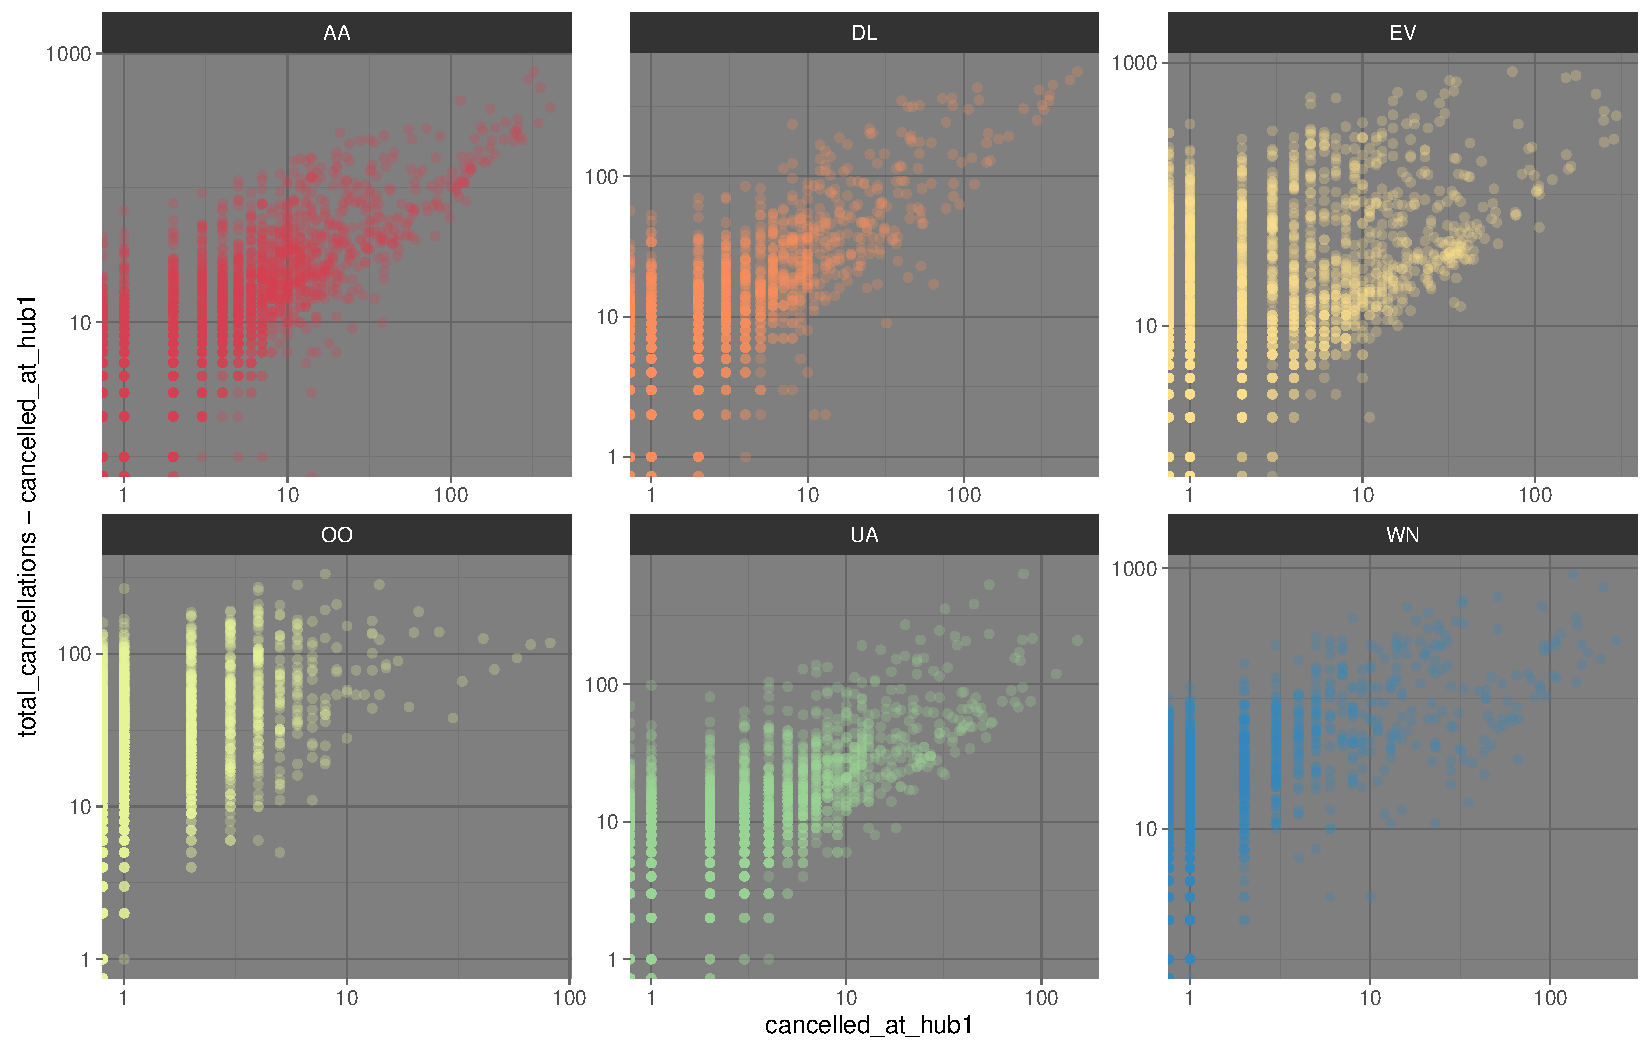
\includegraphics[width=\textwidth]{atlas-post-2008/cancelled-relative-hub1-plot-free-1}
\end{figure*}

\begin{knitrout}
\definecolor{shadecolor}{rgb}{0.969, 0.969, 0.969}\color{fgcolor}\begin{kframe}
\begin{alltt}
\hlstd{cancelled.flights.with.hub.cancelled} \hlopt
  \hlkwd{filter}\hlstd{(UniqueCarrier} \hlopt \hlstd{biggest.carriers)} \hlopt
  \hlkwd{ggplot}\hlstd{(}\hlkwd{aes}\hlstd{(}\hlkwc{x} \hlstd{= cancelled_at_hub2,} \hlkwc{y} \hlstd{= total_cancellations} \hlopt{-} \hlstd{cancelled_at_hub2))} \hlopt{+}
  \hlkwd{geom_point}\hlstd{(}\hlkwd{aes}\hlstd{(}\hlkwc{color} \hlstd{= UniqueCarrier),} \hlkwc{alpha} \hlstd{=} \hlnum{0.25}\hlstd{)} \hlopt{+}
  \hlkwd{scale_color_brewer}\hlstd{(}\hlkwc{palette} \hlstd{=} \hlstr{"Spectral"}\hlstd{)} \hlopt{+}
  \hlkwd{guides}\hlstd{(}\hlkwc{color} \hlstd{=} \hlnum{FALSE}\hlstd{)} \hlopt{+}
  \hlkwd{scale_x_log10}\hlstd{()} \hlopt{+} \hlkwd{scale_y_log10}\hlstd{()} \hlopt{+}
  \hlkwd{facet_wrap}\hlstd{(}\hlopt{~}\hlstd{UniqueCarrier,} \hlkwc{scales} \hlstd{=} \hlstr{"free"}\hlstd{)} \hlopt{+}
  \hlkwd{theme_dark}\hlstd{()}
\end{alltt}
\end{kframe}
\end{knitrout}

\begin{figure*}
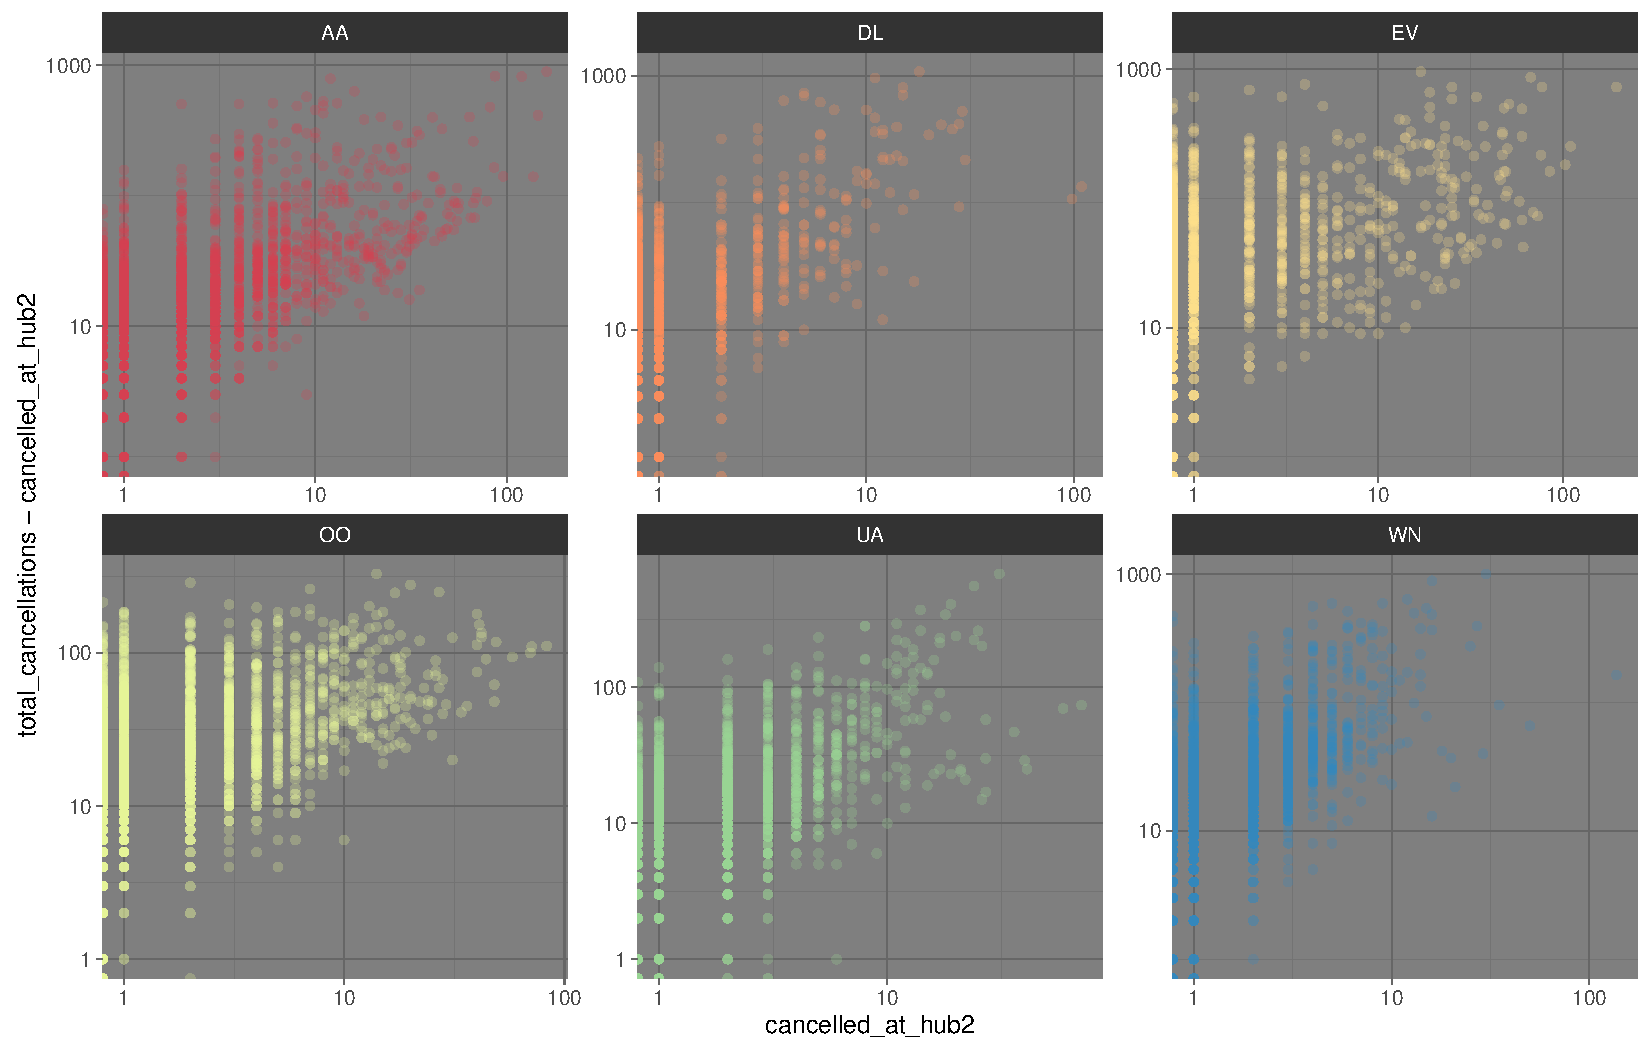
\includegraphics[width=\textwidth]{atlas-post-2008/cancelled-relative-hub2-plot-free-1}
\end{figure*}

% Cancelled at one hub but not others.
\begin{knitrout}
\definecolor{shadecolor}{rgb}{0.969, 0.969, 0.969}\color{fgcolor}\begin{kframe}
\begin{alltt}
\hlstd{cancelled.flights.with.hub.cancelled} \hlopt
  \hlkwd{filter}\hlstd{(UniqueCarrier} \hlopt \hlstd{biggest.carriers)} \hlopt
  \hlkwd{group_by}\hlstd{(Year, Month, DayofMonth)} \hlopt
  \hlkwd{mutate}\hlstd{(}\hlkwc{cancelled_at_hub1_rel_other_hubs} \hlstd{= cancelled_at_hub1} \hlopt{-} \hlkwd{mean}\hlstd{(cancelled_at_hub1),}
         \hlkwc{cancelled_rel_other_carriers} \hlstd{= total_cancellations} \hlopt{-} \hlkwd{mean}\hlstd{(total_cancellations))} \hlopt
  \hlkwd{ggplot}\hlstd{(}\hlkwd{aes}\hlstd{(}\hlkwc{x} \hlstd{= cancelled_at_hub1_rel_other_hubs,} \hlkwc{y} \hlstd{= cancelled_rel_other_carriers))} \hlopt{+}
  \hlkwd{geom_point}\hlstd{(}\hlkwd{aes}\hlstd{(}\hlkwc{color} \hlstd{= UniqueCarrier),} \hlkwc{alpha} \hlstd{=} \hlnum{0.25}\hlstd{)} \hlopt{+}
  \hlkwd{scale_color_brewer}\hlstd{(}\hlkwc{palette} \hlstd{=} \hlstr{"Spectral"}\hlstd{)} \hlopt{+}
  \hlkwd{guides}\hlstd{(}\hlkwc{color} \hlstd{=} \hlnum{FALSE}\hlstd{)} \hlopt{+}
  \hlkwd{facet_wrap}\hlstd{(}\hlopt{~}\hlstd{UniqueCarrier,} \hlkwc{scales} \hlstd{=} \hlstr{"free"}\hlstd{)} \hlopt{+}
  \hlkwd{theme_dark}\hlstd{()}
\end{alltt}
\end{kframe}
\end{knitrout}

\begin{knitrout}
\definecolor{shadecolor}{rgb}{0.969, 0.969, 0.969}\color{fgcolor}\begin{kframe}
\begin{alltt}
\hlstd{cancelled.flights.with.hub.cancelled} \hlopt
  \hlkwd{filter}\hlstd{(UniqueCarrier} \hlopt \hlstd{biggest.carriers)} \hlopt
  \hlkwd{group_by}\hlstd{(Year, Month, DayofMonth)} \hlopt
  \hlkwd{mutate}\hlstd{(}\hlkwc{cancelled_at_hub1_rel_other_hubs} \hlstd{= cancelled_at_hub1} \hlopt{-} \hlkwd{mean}\hlstd{(cancelled_at_hub1),}
         \hlkwc{cancelled_outside_hub_rel_other_carriers} \hlstd{= (total_cancellations} \hlopt{-} \hlstd{cancelled_at_hub1)} \hlopt{-} \hlkwd{mean}\hlstd{(total_cancellations} \hlopt{-} \hlstd{cancelled_at_hub1))} \hlopt
  \hlkwd{ggplot}\hlstd{(}\hlkwd{aes}\hlstd{(}\hlkwc{x} \hlstd{= cancelled_at_hub1_rel_other_hubs,} \hlkwc{y} \hlstd{= cancelled_outside_hub_rel_other_carriers))} \hlopt{+}
  \hlkwd{geom_point}\hlstd{(}\hlkwd{aes}\hlstd{(}\hlkwc{color} \hlstd{= UniqueCarrier),} \hlkwc{alpha} \hlstd{=} \hlnum{0.25}\hlstd{)} \hlopt{+}
  \hlkwd{scale_color_brewer}\hlstd{(}\hlkwc{palette} \hlstd{=} \hlstr{"Spectral"}\hlstd{)} \hlopt{+}
  \hlkwd{guides}\hlstd{(}\hlkwc{color} \hlstd{=} \hlnum{FALSE}\hlstd{)} \hlopt{+}
  \hlkwd{facet_wrap}\hlstd{(}\hlopt{~}\hlstd{UniqueCarrier,} \hlkwc{scales} \hlstd{=} \hlstr{"free"}\hlstd{)} \hlopt{+}
  \hlkwd{theme_dark}\hlstd{()}
\end{alltt}
\end{kframe}
\end{knitrout}

\begin{knitrout}
\definecolor{shadecolor}{rgb}{0.969, 0.969, 0.969}\color{fgcolor}\begin{kframe}
\begin{alltt}
\hlstd{ArrDelays.by.day} \hlkwb{<-}
  \hlstd{flights} \hlopt
  \hlkwd{select}\hlstd{(Year, Month, DayofMonth, ArrDelay)} \hlopt
  \hlkwd{group_by}\hlstd{(Year, Month, DayofMonth)} \hlopt
  \hlkwd{summarise}\hlstd{(}\hlkwc{total_ArrDelay_allcarriers} \hlstd{=} \hlkwd{sum}\hlstd{(ArrDelay,} \hlkwc{na.rm} \hlstd{=} \hlnum{TRUE}\hlstd{))} \hlopt
  \hlkwd{setkey}\hlstd{(Year, Month, DayofMonth)}

\hlstd{ArrDelays.avg.by.day} \hlkwb{<-}
  \hlstd{flights} \hlopt
  \hlkwd{select}\hlstd{(Year, Month, DayofMonth, ArrDelay)} \hlopt
  \hlkwd{group_by}\hlstd{(Year, Month, DayofMonth)} \hlopt
  \hlkwd{summarise}\hlstd{(}\hlkwc{avg_ArrDelay_allcarriers} \hlstd{=} \hlkwd{sum}\hlstd{(ArrDelay,} \hlkwc{na.rm} \hlstd{=} \hlnum{TRUE}\hlstd{)}\hlopt{/}\hlkwd{n}\hlstd{())} \hlopt
  \hlkwd{setkey}\hlstd{(Year, Month, DayofMonth)}

\hlstd{dates.arrdelay.rel.hub} \hlkwb{<-}
  \hlstd{flights} \hlopt
  \hlkwd{select}\hlstd{(Year, Month, DayofMonth, UniqueCarrier, Origin, ArrDelay)} \hlopt
  \hlkwd{setkey}\hlstd{(UniqueCarrier)} \hlopt
  \hlstd{data.table}\hlopt{:::}\hlkwd{merge.data.table}\hlstd{(hub1.by.carrier)} \hlopt
  \hlkwd{group_by}\hlstd{(Year, Month, DayofMonth, UniqueCarrier)} \hlopt
  \hlkwd{summarise}\hlstd{(}\hlkwc{total_arrdelay} \hlstd{=} \hlkwd{sum}\hlstd{(ArrDelay,} \hlkwc{na.rm} \hlstd{=} \hlnum{TRUE}\hlstd{),}
            \hlkwc{arrdelay_at_hub} \hlstd{=} \hlkwd{sum}\hlstd{(ArrDelay} \hlopt{*} \hlstd{(Origin} \hlopt{==} \hlstd{Hub1),} \hlkwc{na.rm} \hlstd{=} \hlnum{TRUE}\hlstd{),}
            \hlkwc{arrdelay_not_at_hub} \hlstd{=} \hlkwd{sum}\hlstd{(ArrDelay} \hlopt{*} \hlstd{(Origin} \hlopt{!=} \hlstd{Hub1),} \hlkwc{na.rm} \hlstd{=} \hlnum{TRUE}\hlstd{))} \hlopt
  \hlkwd{setkey}\hlstd{(Year, Month, DayofMonth)} \hlopt
  \hlstd{data.table}\hlopt{:::}\hlkwd{merge.data.table}\hlstd{(ArrDelays.by.day)}

\hlstd{dates.avg.arrdelay.rel.hub} \hlkwb{<-}
  \hlstd{flights} \hlopt
  \hlkwd{select}\hlstd{(Year, Month, DayofMonth, UniqueCarrier, Origin, ArrDelay)} \hlopt
  \hlkwd{setkey}\hlstd{(UniqueCarrier)} \hlopt
  \hlstd{data.table}\hlopt{:::}\hlkwd{merge.data.table}\hlstd{(hub1.by.carrier)} \hlopt
  \hlkwd{group_by}\hlstd{(Year, Month, DayofMonth, UniqueCarrier)} \hlopt
  \hlkwd{summarise}\hlstd{(}\hlkwc{avg_arrdelay} \hlstd{=} \hlkwd{sum}\hlstd{(ArrDelay,} \hlkwc{na.rm} \hlstd{=} \hlnum{TRUE}\hlstd{)}\hlopt{/}\hlkwd{n}\hlstd{(),}
            \hlkwc{avg_arrdelay_at_hub} \hlstd{=} \hlkwd{sum}\hlstd{(ArrDelay} \hlopt{*} \hlstd{(Origin} \hlopt{==} \hlstd{Hub1),} \hlkwc{na.rm} \hlstd{=} \hlnum{TRUE}\hlstd{)}\hlopt{/}\hlkwd{sum}\hlstd{(Origin} \hlopt{==} \hlstd{Hub1),}
            \hlkwc{avg_arrdelay_not_at_hub} \hlstd{=} \hlkwd{sum}\hlstd{(ArrDelay} \hlopt{*} \hlstd{(Origin} \hlopt{!=} \hlstd{Hub1),} \hlkwc{na.rm} \hlstd{=} \hlnum{TRUE}\hlstd{)} \hlopt{/} \hlkwd{sum}\hlstd{(Origin} \hlopt{!=} \hlstd{Hub1))} \hlopt
  \hlkwd{setkey}\hlstd{(Year, Month, DayofMonth)} \hlopt
  \hlstd{data.table}\hlopt{:::}\hlkwd{merge.data.table}\hlstd{(ArrDelays.avg.by.day)}


\hlstd{dates.arrdelay.rel.hub} \hlopt
  \hlkwd{filter}\hlstd{(UniqueCarrier} \hlopt \hlkwd{select_large_carriers}\hlstd{(}\hlnum{9}\hlstd{))} \hlopt
  \hlkwd{ggplot}\hlstd{(}\hlkwd{aes}\hlstd{(}\hlkwc{x} \hlstd{= total_arrdelay,} \hlkwc{y} \hlstd{= arrdelay_at_hub,} \hlkwc{color} \hlstd{= UniqueCarrier))} \hlopt{+}
  \hlkwd{geom_point}\hlstd{(}\hlkwc{alpha} \hlstd{=} \hlnum{0.33}\hlstd{)} \hlopt{+}
  \hlkwd{facet_wrap}\hlstd{(}\hlopt{~}\hlstd{UniqueCarrier)} \hlopt{+}
  \hlkwd{theme_dark}\hlstd{()} \hlopt{+}
  \hlkwd{scale_color_brewer}\hlstd{(}\hlkwc{palette} \hlstd{=} \hlstr{"Spectral"}\hlstd{)}
\end{alltt}
\end{kframe}
\end{knitrout}

\begin{knitrout}
\definecolor{shadecolor}{rgb}{0.969, 0.969, 0.969}\color{fgcolor}\begin{kframe}
\begin{alltt}
\hlstd{dates.avg.arrdelay.rel.hub} \hlopt
  \hlkwd{filter}\hlstd{(UniqueCarrier} \hlopt \hlkwd{select_large_carriers}\hlstd{(}\hlnum{9}\hlstd{))} \hlopt
  \hlkwd{merge}\hlstd{(nycflights.airlines,} \hlkwc{by} \hlstd{=} \hlstr{"UniqueCarrier"}\hlstd{)} \hlopt
  \hlkwd{ggplot}\hlstd{(}\hlkwd{aes}\hlstd{(}\hlkwc{x} \hlstd{= avg_arrdelay_at_hub,} \hlkwc{y} \hlstd{= avg_arrdelay_not_at_hub,} \hlkwc{color} \hlstd{= UniqueCarrier))} \hlopt{+}
  \hlkwd{geom_point}\hlstd{(}\hlkwc{alpha} \hlstd{=} \hlnum{0.33}\hlstd{)} \hlopt{+}
  \hlkwd{facet_wrap}\hlstd{(}\hlopt{~}\hlstd{short_name)} \hlopt{+}
  \hlkwd{theme_dark}\hlstd{()} \hlopt{+}
  \hlkwd{scale_color_brewer}\hlstd{(}\hlkwc{palette} \hlstd{=} \hlstr{"Spectral"}\hlstd{,} \hlkwc{guide} \hlstd{=} \hlnum{FALSE}\hlstd{)}
\end{alltt}
\end{kframe}
\end{knitrout}

\begin{knitrout}
\definecolor{shadecolor}{rgb}{0.969, 0.969, 0.969}\color{fgcolor}\begin{kframe}
\begin{alltt}
\hlstd{dates.avg.arrdelay.rel.hub} \hlopt
  \hlkwd{filter}\hlstd{(UniqueCarrier} \hlopt \hlkwd{select_large_carriers}\hlstd{(}\hlnum{9}\hlstd{))} \hlopt
  \hlkwd{merge}\hlstd{(nycflights.airlines,} \hlkwc{by} \hlstd{=} \hlstr{"UniqueCarrier"}\hlstd{)} \hlopt
  \hlkwd{ggplot}\hlstd{(}\hlkwd{aes}\hlstd{(}\hlkwc{x} \hlstd{= avg_arrdelay_at_hub,} \hlkwc{y} \hlstd{= avg_arrdelay_not_at_hub,} \hlkwc{color} \hlstd{= UniqueCarrier))} \hlopt{+}
  \hlkwd{geom_point}\hlstd{(}\hlkwc{alpha} \hlstd{=} \hlnum{0.33}\hlstd{)} \hlopt{+}
  \hlkwd{facet_wrap}\hlstd{(}\hlopt{~}\hlstd{short_name,} \hlkwc{scales} \hlstd{=} \hlstr{"free"}\hlstd{)} \hlopt{+}
  \hlkwd{theme_dark}\hlstd{()} \hlopt{+}
  \hlkwd{scale_color_brewer}\hlstd{(}\hlkwc{palette} \hlstd{=} \hlstr{"Spectral"}\hlstd{,} \hlkwc{guide} \hlstd{=} \hlnum{FALSE}\hlstd{)}
\end{alltt}
\end{kframe}
\end{knitrout}

\begin{knitrout}
\definecolor{shadecolor}{rgb}{0.969, 0.969, 0.969}\color{fgcolor}\begin{kframe}
\begin{alltt}
\hlstd{dates.avg.arrdelay.rel.hub} \hlopt
  \hlkwd{filter}\hlstd{(UniqueCarrier} \hlopt \hlkwd{select_large_carriers}\hlstd{(}\hlnum{9}\hlstd{))} \hlopt
  \hlkwd{merge}\hlstd{(nycflights.airlines,} \hlkwc{by} \hlstd{=} \hlstr{"UniqueCarrier"}\hlstd{)} \hlopt
  \hlkwd{ggplot}\hlstd{(}\hlkwd{aes}\hlstd{(}\hlkwc{x} \hlstd{= avg_arrdelay_at_hub} \hlopt{-} \hlstd{avg_ArrDelay_allcarriers,} \hlkwc{y} \hlstd{= avg_arrdelay_not_at_hub} \hlopt{-} \hlstd{avg_ArrDelay_allcarriers,} \hlkwc{color} \hlstd{= UniqueCarrier))} \hlopt{+}
  \hlkwd{geom_point}\hlstd{(}\hlkwc{alpha} \hlstd{=} \hlnum{0.33}\hlstd{)} \hlopt{+}
  \hlkwd{facet_wrap}\hlstd{(}\hlopt{~}\hlstd{short_name)} \hlopt{+}
  \hlkwd{theme_dark}\hlstd{()} \hlopt{+}
  \hlkwd{geom_abline}\hlstd{(}\hlkwc{slope} \hlstd{=} \hlnum{1}\hlstd{,} \hlkwc{color} \hlstd{=} \hlstr{"white"}\hlstd{)} \hlopt{+}
  \hlkwd{scale_color_brewer}\hlstd{(}\hlkwc{palette} \hlstd{=} \hlstr{"Spectral"}\hlstd{,} \hlkwc{guide} \hlstd{=} \hlnum{FALSE}\hlstd{)}
\end{alltt}
\end{kframe}
\end{knitrout}

\begin{knitrout}
\definecolor{shadecolor}{rgb}{0.969, 0.969, 0.969}\color{fgcolor}\begin{kframe}
\begin{alltt}
\hlstd{dates.avg.arrdelay.rel.hub} \hlopt
  \hlkwd{filter}\hlstd{(UniqueCarrier} \hlopt \hlkwd{select_large_carriers}\hlstd{(}\hlnum{9}\hlstd{))} \hlopt
  \hlkwd{merge}\hlstd{(nycflights.airlines,} \hlkwc{by} \hlstd{=} \hlstr{"UniqueCarrier"}\hlstd{)} \hlopt
  \hlkwd{ggplot}\hlstd{(}\hlkwd{aes}\hlstd{(}\hlkwc{x} \hlstd{= avg_arrdelay_at_hub} \hlopt{-} \hlstd{avg_ArrDelay_allcarriers,} \hlkwc{y} \hlstd{= avg_arrdelay_not_at_hub} \hlopt{-} \hlstd{avg_ArrDelay_allcarriers,} \hlkwc{color} \hlstd{= UniqueCarrier))} \hlopt{+}
  \hlkwd{geom_point}\hlstd{(}\hlkwc{alpha} \hlstd{=} \hlnum{0.33}\hlstd{)} \hlopt{+}
  \hlkwd{facet_wrap}\hlstd{(}\hlopt{~}\hlstd{short_name,} \hlkwc{scales} \hlstd{=} \hlstr{"free"}\hlstd{)} \hlopt{+}
  \hlkwd{theme_dark}\hlstd{()} \hlopt{+}
  \hlkwd{scale_color_manual}\hlstd{(}\hlkwc{values} \hlstd{= carrier.colors)}
\end{alltt}
\end{kframe}
\end{knitrout}

\begin{knitrout}
\definecolor{shadecolor}{rgb}{0.969, 0.969, 0.969}\color{fgcolor}\begin{kframe}
\begin{alltt}
\hlstd{city.market.decoder} \hlkwb{<-} \hlkwd{fread}\hlstd{(}\hlstr{"../metadata/L_CITY_MARKET_ID.csv"}\hlstd{,} \hlkwc{verbose} \hlstd{=} \hlnum{TRUE}\hlstd{,} \hlkwc{colClasses} \hlstd{=} \hlkwd{c}\hlstd{(}\hlstr{"integer"}\hlstd{,} \hlstr{"character"}\hlstd{))}
\end{alltt}
\begin{verbatim}
## Input contains no \n. Taking this to be a filename to open
## File opened, filesize is 0.000153 GB.
## Memory mapping ... ok
## Detected eol as \r\n (CRLF) in that order, the Windows standard.
## Positioned on line 1 after skip or autostart
## This line is the autostart and not blank so searching up for the last non-blank ... line 1
## Detecting sep ... ','
## Detected 2 columns. Longest stretch was from line 1 to line 30
## Starting data input on line 1 (either column names or first row of data). First 10 characters: Code,Descr
## All the fields on line 1 are character fields. Treating as the column names.
## Count of eol: 5750 (including 1 at the end)
## Count of sep: 11506
## nrow = MIN( nsep [11506] / ncol [2] -1, neol [5750] - nblank [1] ) = 5749
## Type codes (   first 5 rows): 44
## Type codes (+ middle 5 rows): 44
## Type codes (+   last 5 rows): 44
\end{verbatim}


{\ttfamily\noindent\color{warningcolor}{\#\# Warning in fread("{}../metadata/L\_CITY\_MARKET\_ID.csv"{}, verbose = TRUE, colClasses = c("{}integer"{}, : Column 1 ('Code') has been detected as type 'character'. Ignoring request from colClasses to read as 'integer' (a lower type) since NAs (or loss of precision) may result.}}\begin{verbatim}
## Type codes: 44 (after applying colClasses and integer64)
## Type codes: 44 (after applying drop or select (if supplied)
## Allocating 2 column slots (2 - 0 dropped)
## Read 5749 rows. Exactly what was estimated and allocated up front
##    0.000s (  0%) Memory map (rerun may be quicker)
##    0.000s (  0%) sep and header detection
##    0.000s (  0%) Count rows (wc -l)
##    0.000s (  0%) Column type detection (first, middle and last 5 rows)
##    0.000s (  0%) Allocation of 5749x2 result (xMB) in RAM
##    0.003s (100%) Reading data
##    0.000s (  0%) Allocation for type bumps (if any), including gc time if triggered
##    0.000s (  0%) Coercing data already read in type bumps (if any)
##    0.000s (  0%) Changing na.strings to NA
##    0.003s        Total
\end{verbatim}
\begin{alltt}
\hlstd{city.market.decoder[,Code} \hlkwb{:=} \hlkwd{as.integer}\hlstd{(Code)]}
\hlstd{city.market.volumes} \hlkwb{<-}
  \hlstd{flights} \hlopt
  \hlkwd{select}\hlstd{(OriginCityMarketID)} \hlopt
  \hlkwd{count}\hlstd{(OriginCityMarketID)} \hlopt
  \hlkwd{merge}\hlstd{(city.market.decoder,} \hlkwc{by.x} \hlstd{=} \hlstr{"OriginCityMarketID"}\hlstd{,} \hlkwc{by.y} \hlstd{=} \hlstr{"Code"}\hlstd{)} \hlopt
  \hlkwd{arrange}\hlstd{(n)}
\end{alltt}
\end{kframe}
\end{knitrout}

\begin{knitrout}
\definecolor{shadecolor}{rgb}{0.969, 0.969, 0.969}\color{fgcolor}\begin{kframe}
\begin{alltt}
\hlstd{city.market.volumes.2014} \hlkwb{<-}
  \hlstd{flights[Year} \hlopt{==} \hlnum{2014}\hlstd{,} \hlkwd{.}\hlstd{(}\hlkwc{n} \hlstd{= .N),} \hlkwc{by} \hlstd{= OriginCityMarketID]} \hlopt
  \hlkwd{filter}\hlstd{(n} \hlopt{>=} \hlkwd{nth}\hlstd{(n,} \hlnum{8}\hlstd{,} \hlkwc{order_by} \hlstd{=} \hlopt{-}\hlstd{n))} \hlopt
  \hlkwd{merge}\hlstd{(city.market.decoder,} \hlkwc{by.x} \hlstd{=} \hlstr{"OriginCityMarketID"}\hlstd{,} \hlkwc{by.y} \hlstd{=} \hlstr{"Code"}\hlstd{)} \hlopt
  \hlkwd{arrange}\hlstd{(}\hlkwd{desc}\hlstd{(n))}

\hlstd{flights[,}\hlkwd{.}\hlstd{(}\hlkwc{n} \hlstd{= .N),} \hlkwc{by} \hlstd{=} \hlkwd{list}\hlstd{(Year, OriginCityMarketID)]} \hlopt
  \hlkwd{merge}\hlstd{(city.market.decoder,} \hlkwc{by.x} \hlstd{=} \hlstr{"OriginCityMarketID"}\hlstd{,} \hlkwc{by.y} \hlstd{=} \hlstr{"Code"}\hlstd{)} \hlopt
  \hlkwd{group_by}\hlstd{(Year)} \hlopt
  \hlkwd{filter}\hlstd{(n} \hlopt{>=} \hlkwd{nth}\hlstd{(n,} \hlnum{8}\hlstd{,} \hlkwc{order_by} \hlstd{=} \hlopt{-}\hlstd{n))} \hlopt
  \hlstd{tbl_df} \hlopt
  \hlkwd{mutate}\hlstd{(}\hlkwc{Description} \hlstd{=} \hlkwd{factor}\hlstd{(Description))} \hlopt
  \hlkwd{mutate}\hlstd{(}\hlkwc{Description} \hlstd{=} \hlkwd{factor}\hlstd{(Description,}
                              \hlkwc{levels} \hlstd{= city.market.volumes.2014}\hlopt{$}\hlstd{Description,}
                              \hlkwc{labels} \hlstd{=} \hlkwd{gsub}\hlstd{(}\hlstr{", [A-Z]\{2\}.*$"}\hlstd{,} \hlstr{""}\hlstd{, city.market.volumes.2014}\hlopt{$}\hlstd{Description)))} \hlopt
  \hlkwd{filter}\hlstd{(Year} \hlopt{<} \hlkwd{max}\hlstd{(Year))} \hlopt
  \hlstd{\{}
  \hlkwd{ggplot}\hlstd{(.,} \hlkwd{aes}\hlstd{(}\hlkwc{x} \hlstd{= Year,} \hlkwc{y} \hlstd{= n,} \hlkwc{group} \hlstd{= Description,} \hlkwc{color} \hlstd{= Description))} \hlopt{+}
  \hlkwd{geom_line}\hlstd{()} \hlopt{+}
  \hlkwd{geom_dl}\hlstd{(}\hlkwc{method} \hlstd{=} \hlstr{"last.points"}\hlstd{,} \hlkwd{aes}\hlstd{(}\hlkwc{label} \hlstd{= Description))} \hlopt{+}
  \hlkwd{scale_color_brewer}\hlstd{(}\hlkwc{palette} \hlstd{=} \hlstr{"Spectral"}\hlstd{)} \hlopt{+}
  \hlkwd{theme}\hlstd{(}\hlkwc{legend.position} \hlstd{=} \hlstr{"none"}\hlstd{)} \hlopt{+}
  \hlkwd{scale_x_continuous}\hlstd{(}\hlkwc{limits} \hlstd{=} \hlkwd{c}\hlstd{(}\hlkwd{min}\hlstd{(.}\hlopt{$}\hlstd{Year),} \hlkwd{max}\hlstd{(.}\hlopt{$}\hlstd{Year)}  \hlopt{+} \hlstd{(}\hlkwd{max}\hlstd{(.}\hlopt{$}\hlstd{Year)} \hlopt{-} \hlkwd{min}\hlstd{(.}\hlopt{$}\hlstd{Year))}\hlopt{*}\hlnum{0.15}\hlstd{))}
  \hlstd{\}}
\end{alltt}
\end{kframe}
\end{knitrout}

\begin{knitrout}
\definecolor{shadecolor}{rgb}{0.969, 0.969, 0.969}\color{fgcolor}\begin{kframe}
\begin{alltt}
\hlstd{city.market.volumes.2014} \hlkwb{<-}
  \hlstd{flights[Year} \hlopt{==} \hlnum{2014}\hlstd{,} \hlkwd{.}\hlstd{(}\hlkwc{n} \hlstd{= .N),} \hlkwc{by} \hlstd{= OriginCityMarketID]} \hlopt
  \hlkwd{filter}\hlstd{(n} \hlopt{>=} \hlkwd{nth}\hlstd{(n,} \hlnum{8}\hlstd{,} \hlkwc{order_by} \hlstd{=} \hlopt{-}\hlstd{n))} \hlopt
  \hlkwd{merge}\hlstd{(city.market.decoder,} \hlkwc{by.x} \hlstd{=} \hlstr{"OriginCityMarketID"}\hlstd{,} \hlkwc{by.y} \hlstd{=} \hlstr{"Code"}\hlstd{)} \hlopt
  \hlkwd{arrange}\hlstd{(}\hlkwd{desc}\hlstd{(n))}

\hlstd{flights[,}\hlkwd{.}\hlstd{(}\hlkwc{n} \hlstd{= .N),} \hlkwc{by} \hlstd{=} \hlkwd{list}\hlstd{(Week, OriginCityMarketID)]} \hlopt
  \hlkwd{merge}\hlstd{(city.market.decoder,} \hlkwc{by.x} \hlstd{=} \hlstr{"OriginCityMarketID"}\hlstd{,} \hlkwc{by.y} \hlstd{=} \hlstr{"Code"}\hlstd{)} \hlopt
  \hlkwd{group_by}\hlstd{(Week)} \hlopt
  \hlkwd{filter}\hlstd{(OriginCityMarketID} \hlopt \hlstd{city.market.volumes.2014}\hlopt{$}\hlstd{OriginCityMarketID)} \hlopt
  \hlstd{tbl_df} \hlopt
  \hlkwd{mutate}\hlstd{(}\hlkwc{Description} \hlstd{=} \hlkwd{factor}\hlstd{(Description))} \hlopt
  \hlkwd{mutate}\hlstd{(}\hlkwc{Description} \hlstd{=} \hlkwd{factor}\hlstd{(Description,}
                              \hlkwc{levels} \hlstd{= city.market.volumes.2014}\hlopt{$}\hlstd{Description,}
                              \hlkwc{labels} \hlstd{=} \hlkwd{gsub}\hlstd{(}\hlstr{", [A-Z]\{2\}.*$"}\hlstd{,} \hlstr{""}\hlstd{, city.market.volumes.2014}\hlopt{$}\hlstd{Description)))} \hlopt

  \hlkwd{filter}\hlstd{(Week} \hlopt{<} \hlkwd{max}\hlstd{(Week)} \hlopt{&} \hlstd{Week} \hlopt{>} \hlkwd{min}\hlstd{(Week))} \hlopt
  \hlkwd{mutate}\hlstd{(}\hlkwc{Description.label} \hlstd{=} \hlkwd{ifelse}\hlstd{(Week} \hlopt{==} \hlkwd{max}\hlstd{(Week),} \hlkwd{as.character}\hlstd{(Description),} \hlnum{NA_character_}\hlstd{))} \hlopt
  \hlstd{\{}
    \hlkwd{ggplot}\hlstd{(.,} \hlkwd{aes}\hlstd{(}\hlkwc{x} \hlstd{= Week,} \hlkwc{y} \hlstd{= n,} \hlkwc{group} \hlstd{= Description,} \hlkwc{color} \hlstd{= Description))} \hlopt{+}
      \hlkwd{geom_line}\hlstd{()} \hlopt{+}
      \hlcom{# geom_text_repel(aes(x = Week, label = Description.label), size = 6, fontface = "bold") + }
      \hlcom{# geom_dl(method = "last.points", aes(label = Description)) +}
      \hlkwd{geom_text}\hlstd{(}\hlkwd{aes}\hlstd{(}\hlkwc{label} \hlstd{= Description.label),} \hlkwc{hjust} \hlstd{=} \hlnum{0}\hlstd{,} \hlkwc{check_overlap} \hlstd{=} \hlnum{TRUE}\hlstd{)} \hlopt{+}
      \hlkwd{scale_color_brewer}\hlstd{(}\hlkwc{palette} \hlstd{=} \hlstr{"Spectral"}\hlstd{)} \hlopt{+}
      \hlkwd{theme}\hlstd{(}\hlkwc{legend.position} \hlstd{=} \hlstr{"none"}\hlstd{)} \hlopt{+}
      \hlkwd{annotate}\hlstd{(}\hlstr{"blank"}\hlstd{,} \hlkwc{x} \hlstd{=} \hlkwd{max}\hlstd{(.}\hlopt{$}\hlstd{Week)} \hlopt{+} \hlnum{50}\hlstd{,} \hlkwc{y} \hlstd{=} \hlkwd{mean}\hlstd{(.}\hlopt{$}\hlstd{n))} \hlopt{+}
      \hlkwd{theme_dark}\hlstd{()}

  \hlstd{\}}
\end{alltt}


{\ttfamily\noindent\color{warningcolor}{\#\# Warning: Removed 3240 rows containing missing values (geom\_text).}}\end{kframe}
\end{knitrout}

\begin{knitrout}
\definecolor{shadecolor}{rgb}{0.969, 0.969, 0.969}\color{fgcolor}\begin{kframe}
\begin{alltt}
\hlstd{corridor.volumes.by.week} \hlkwb{<-}
  \hlstd{flights[, Corridor} \hlkwb{:=} \hlkwd{pmin}\hlstd{(}\hlkwd{paste0}\hlstd{(OriginCityMarketID,} \hlstr{"-"}\hlstd{, DestCityMarketID),}
                             \hlkwd{paste0}\hlstd{(DestCityMarketID,} \hlstr{"-"}\hlstd{, OriginCityMarketID))][,}\hlkwd{.}\hlstd{(}\hlkwc{n} \hlstd{= .N),}
                                                                                 \hlkwc{by} \hlstd{=} \hlkwd{list}\hlstd{(Week,Corridor)][}\hlkwd{order}\hlstd{(}\hlopt{-}\hlstd{n)]}
\end{alltt}
\end{kframe}
\end{knitrout}

\begin{knitrout}
\definecolor{shadecolor}{rgb}{0.969, 0.969, 0.969}\color{fgcolor}\begin{kframe}
\begin{alltt}
\hlstd{corridor.volumes.by.week} \hlkwb{<-}
  \hlstd{flights[, Corridor} \hlkwb{:=} \hlkwd{sprintf}\hlstd{(}\hlstr{"%s-%s"}\hlstd{,}
                                \hlkwd{pmin}\hlstd{(OriginCityMarketID, DestCityMarketID),}
                                \hlkwd{pmax}\hlstd{(OriginCityMarketID, DestCityMarketID))][,}\hlkwd{.}\hlstd{(}\hlkwc{n} \hlstd{= .N),}
                                                                             \hlkwc{by} \hlstd{=} \hlkwd{list}\hlstd{(Week,Corridor)][}\hlkwd{order}\hlstd{(}\hlopt{-}\hlstd{n)]}
\end{alltt}
\end{kframe}
\end{knitrout}



\begin{knitrout}
\definecolor{shadecolor}{rgb}{0.969, 0.969, 0.969}\color{fgcolor}\begin{kframe}
\begin{alltt}
\hlstd{Corridors} \hlkwb{<-}
  \hlstd{data.table}\hlopt{::}\hlkwd{CJ}\hlstd{(}\hlkwc{OriginCityMarketID} \hlstd{= city.market.decoder}\hlopt{$}\hlstd{Code,}
                 \hlkwc{DestCityMarketID} \hlstd{= city.market.decoder}\hlopt{$}\hlstd{Code)} \hlopt
  \hlkwd{merge}\hlstd{(city.market.decoder,} \hlkwc{by.x} \hlstd{=} \hlstr{"OriginCityMarketID"}\hlstd{,} \hlkwc{by.y} \hlstd{=} \hlstr{"Code"}\hlstd{)} \hlopt
  \hlkwd{setnames}\hlstd{(}\hlstr{"Description"}\hlstd{,} \hlstr{"OriginCityMarketID_DS"}\hlstd{)} \hlopt
  \hlkwd{merge}\hlstd{(city.market.decoder,} \hlkwc{by.x} \hlstd{=} \hlstr{"DestCityMarketID"}\hlstd{,} \hlkwc{by.y} \hlstd{=} \hlstr{"Code"}\hlstd{)} \hlopt
  \hlkwd{setnames}\hlstd{(}\hlstr{"Description"}\hlstd{,} \hlstr{"DestCityMarketID_DS"}\hlstd{)}

\hlstd{Corridors[,Corridor} \hlkwb{:=} \hlkwd{paste0}\hlstd{(OriginCityMarketID,} \hlstr{"-"}\hlstd{, DestCityMarketID)]}
\hlstd{Corridors[,Corridor_DS} \hlkwb{:=} \hlkwd{paste0}\hlstd{(OriginCityMarketID_DS,} \hlstr{"-"}\hlstd{, DestCityMarketID_DS)]}
\hlstd{Corridors} \hlopt \hlkwd{select}\hlstd{(Corridor, Corridor_DS)} \hlopt \hlkwd{setkey}\hlstd{(Corridor)}
\hlkwd{gc}\hlstd{(T,T)}
\end{alltt}
\begin{verbatim}
##              used    (Mb) gc trigger    (Mb)   max used    (Mb)
## Ncells   66766183  3565.7   90464440  4831.4   66766183  3565.7
## Vcells 3058649203 23335.7 5077629258 38739.3 3058649203 23335.7
\end{verbatim}
\end{kframe}
\end{knitrout}

\begin{knitrout}
\definecolor{shadecolor}{rgb}{0.969, 0.969, 0.969}\color{fgcolor}\begin{kframe}
\begin{alltt}
\hlstd{corridor.volumes} \hlkwb{<-}
  \hlstd{corridor.volumes.by.week} \hlopt
  \hlkwd{group_by}\hlstd{(Corridor)} \hlopt
  \hlkwd{summarise}\hlstd{(}\hlkwc{total_volume} \hlstd{=} \hlkwd{sum}\hlstd{(n))} \hlopt
  \hlkwd{arrange}\hlstd{(}\hlkwd{desc}\hlstd{(total_volume))}

\hlstd{corridor.volumes.by.week} \hlopt
  \hlkwd{filter}\hlstd{(Corridor} \hlopt \hlstd{corridor.volumes}\hlopt{$}\hlstd{Corridor[}\hlnum{1}\hlopt{:}\hlnum{10}\hlstd{])} \hlopt
  \hlkwd{setkey}\hlstd{(Corridor)} \hlopt
  \hlkwd{merge}\hlstd{(Corridors)} \hlopt
  \hlkwd{mutate}\hlstd{(}\hlkwc{Corridor_DS_x} \hlstd{=} \hlkwd{gsub}\hlstd{(}\hlstr{"^([A-Z].+),.*-([A-Z].+),.*$"}\hlstd{,} \hlstr{"\textbackslash{}\textbackslash{}1-\textbackslash{}\textbackslash{}2"}\hlstd{, Corridor_DS))} \hlopt
  \hlkwd{filter}\hlstd{(Week} \hlopt{<} \hlkwd{max}\hlstd{(Week))} \hlopt
  \hlkwd{group_by}\hlstd{(Corridor)} \hlopt
  \hlkwd{mutate}\hlstd{(}\hlkwc{maxn} \hlstd{=} \hlkwd{max}\hlstd{(n))} \hlopt
  \hlstd{ungroup} \hlopt
  \hlkwd{mutate}\hlstd{(}\hlkwc{Facet} \hlstd{=} \hlkwd{rank}\hlstd{(maxn)} \hlopt \hlnum{5}\hlstd{)} \hlopt
  \hlkwd{ggplot}\hlstd{(}\hlkwd{aes}\hlstd{(}\hlkwc{x} \hlstd{= Week,} \hlkwc{y} \hlstd{= n,} \hlkwc{group} \hlstd{= Corridor_DS_x,} \hlkwc{color} \hlstd{= Corridor_DS_x))} \hlopt{+}
  \hlkwd{geom_line}\hlstd{()} \hlopt{+}
  \hlkwd{scale_x_continuous}\hlstd{(}\hlkwc{limits} \hlstd{=} \hlkwd{c}\hlstd{(}\hlnum{0}\hlstd{,} \hlnum{450}\hlstd{))} \hlopt{+}
  \hlkwd{geom_dl}\hlstd{(}\hlkwc{method} \hlstd{=} \hlstr{"last.points"}\hlstd{,} \hlkwd{aes}\hlstd{(}\hlkwc{label} \hlstd{= Corridor_DS_x))} \hlopt{+}
  \hlkwd{facet_grid}\hlstd{(Facet} \hlopt{~} \hlstd{.)}
\end{alltt}
\end{kframe}
\end{knitrout}

COMPILATION TIME: 11.5616566181183
\begin{knitrout}
\definecolor{shadecolor}{rgb}{0.969, 0.969, 0.969}\color{fgcolor}\begin{kframe}
\begin{alltt}
\hlstd{COMPILATION.TIME} \hlkwb{<-} \hlkwd{round}\hlstd{(}\hlkwd{difftime}\hlstd{(}\hlkwd{Sys.time}\hlstd{(), START.TIME,} \hlkwc{units} \hlstd{=} \hlstr{"mins"}\hlstd{),} \hlnum{1}\hlstd{)}
\hlkwd{write}\hlstd{(}\hlstr{"======="}\hlstd{,}
\hlkwc{file} \hlstd{=} \hlstr{"analysis-post-2008-CHUNKTIMINGS.txt"}\hlstd{,}
\hlkwc{append} \hlstd{=} \hlnum{TRUE}\hlstd{)}
\hlkwd{write}\hlstd{(}\hlkwd{paste0}\hlstd{(}\hlstr{"Compilation time: "}\hlstd{, COMPILATION.TIME),}
      \hlkwc{file} \hlstd{=} \hlstr{"analysis-post-2008-CHUNKTIMINGS.txt"}\hlstd{,}
      \hlkwc{append} \hlstd{=} \hlnum{TRUE}\hlstd{)}
\hlstd{finished} \hlkwb{<-} \hlnum{TRUE}
\end{alltt}
\end{kframe}
\end{knitrout}
\end{document}
